\documentclass[10pt]{article}
\usepackage[utf8]{inputenc}
\usepackage[english]{babel}
\usepackage[font=small,labelfont=bf]{caption}
\usepackage{geometry}
\usepackage[sort&compress, numbers]{natbib}
\usepackage{pxfonts}
\usepackage{graphicx}
\usepackage{setspace}
\usepackage{hyperref}
\usepackage{lineno}

\usepackage{xcolor}

% supplemental tables
\newcommand{\questions}{1}
\newcommand{\topics}{2}
\newcommand{\matchTab}{3}

% supplemental figures
\newcommand{\topicWordWeights}{1}
\newcommand{\topicWeights}{2}
\newcommand{\forcesCorrs}{3}
\newcommand{\bosCorrs}{4}
\newcommand{\jaccard}{5}
\newcommand{\ldaVsBERT}{6}
\newcommand{\individualKnowledgeMapsA}{7}
\newcommand{\individualKnowledgeMapsB}{8}
\newcommand{\individualKnowledgeMapsC}{9}
\newcommand{\individualLearningMapsA}{10}
\newcommand{\individualLearningMapsB}{11}

\newcommand{\U}{{\fontfamily{serif}\selectfont\ensuremath{\mathrm{U}}}}


% simple command for inline comments
\newcommand{\comment}[1]{}
% italicize section names in \nameref and place in \mbox to prevent bug when
% text is split across lines or pages
\NewCommandCopy{\oldnameref}{\nameref}
\renewcommand{\nameref}[1]{\mbox{\textit{\oldnameref{#1}}}}

\doublespacing
\linenumbers

\title{Text embedding models yield high-resolution insights into conceptual
knowledge from short multiple-choice quizzes}

\author{Paxton C. Fitzpatrick\textsuperscript{1},
Andrew C. Heusser\textsuperscript{1, 2}, and Jeremy R.
Manning\textsuperscript{1, *}\\\small{\textsuperscript{1}Department of Psychological and Brain Sciences}\\\small{Dartmouth College, Hanover, NH 03755, USA}\\\small{\textsuperscript{2}Akili Interactive Labs}\\\small{Boston, MA 02110, USA}\\\small{\textsuperscript{*}Corresponding author:
Jeremy.R.Manning@Dartmouth.edu}}

\date{}

\begin{document}
\maketitle

\begin{abstract}\noindent We develop a mathematical framework, based on natural
language processing models, for tracking and characterizing the acquisition of
conceptual knowledge. Our approach embeds each concept in a high-dimensional
representation space, where nearby coordinates reflect similar or related
concepts. We test our approach using behavioral data from participants who
answered small sets of multiple-choice quiz questions interleaved between
watching two course videos from the Khan Academy platform. We apply our
framework to the videos' transcripts and the text of the quiz questions to
quantify the content of each moment of video and each quiz question. We use
these embeddings, along with participants' quiz responses, to track how the
learners' knowledge changed after watching each video. Our findings show how a
small set of quiz questions may be used to obtain rich and meaningful
high-resolution insights into what each learner knows, and how their knowledge
changes over time as they learn.

\textbf{Keywords: education, learning, knowledge, concepts, natural language processing}

\end{abstract}


\section*{Introduction}

Suppose that a teacher had access to a complete, tangible ``map'' of everything
a student knows. Defining what such a map might even look like, let alone how it
might be constructed or filled in, is itself a non-trivial problem. But if a
teacher \textit{were} to gain access to such a map, how might it change their
ability to teach that student? Perhaps they might start by checking how well
the student knows the to-be-learned information already, or how much they know
about related concepts. For some students, they could potentially optimize
their teaching efforts to maximize efficiency by focusing primarily on
not-yet-known content. For other students (or other content areas), it might be
more effective to optimize for direct connections between already known content
and new material. Observing how the student's knowledge changed over time, in
response to their teaching, could also help to guide the teacher towards the
most effective strategy for that individual student.

A common approach to assessing a student's knowledge is to present them with a
set of quiz questions, calculate the proportion they answer correctly, and
provide them with feedback in the form of a simple numeric or letter grade.
While such a grade can provide \textit{some} indication of whether the student
has mastered the to-be-learned material, any univariate measure of performance
on a complex task sacrifices certain relevant information, risks conflating
underlying factors, and so on. For example, consider the relative utility of
the theoretical map described above that characterizes a student's knowledge in
detail, versus a single annotation saying that the student answered 85\% of
their quiz questions correctly, or that they received a `B'. Here, we show that
the same quiz data required to compute proportion-correct scores or letter
grades can instead be used to obtain far more detailed insights into what a
student knew at the time they took the quiz.

Designing and building procedures and tools for mapping out knowledge touches
on deep questions about what it means to learn. For example, how do we acquire
conceptual knowledge? Memorizing course lectures or textbook chapters by rote
can lead to the superficial \textit{appearance} of understanding the underlying
content, but achieving true conceptual understanding seems to require something
deeper and richer. Does conceptual understanding entail connecting newly
acquired information to the scaffolding of one's existing knowledge or
experience~\citep{BlayEtal06,CaraMaho03, ConsEtal16, DeacEtal04, SimoEtal04,
HuebWill18}? Or weaving a lecture's atomic elements (e.g., its component words)
into a structured network that describes how those individual elements are
related~\citep{LeeChen22, vanPEtal21}? Conceptual understanding could also
involve building a mental model that transcends the meanings of those
individual atomic elements by reflecting the deeper meaning underlying the
gestalt whole~\citep{Kint70, Macl05, ScotEtal07, TulcEtal23}.

The difference between ``understanding'' and ``memorizing,'' as framed
by researchers in education, cognitive psychology, and cognitive
neuroscience~\citep[e.g.,][]{Kato40, Gall00, ScotEtal07, HallGree08,
  Macl05}, has profound analogs in the fields of natural language
processing and natural language understanding. For example,
considering the raw contents of a document (e.g., its constituent
symbols, letters, and words) might provide some clues as to what the
document is about, just as memorizing a passage might provide some
ability to answer simple questions about it. However, text embedding
models~\citep[e.g.,][]{LandDuma97, DeerEtal90, BleiEtal03,
  BleiLaff06, MikoEtal13a, CerEtal18, BrowEtal20, ViswEtal17} also
attempt to capture the deeper meaning \textit{underlying} those atomic
elements. These models consider not only the co-occurrences of those
elements within and across documents, but (in many cases) also
patterns in how those elements appear across different scales (e.g.,
sentences, paragraphs, chapters, etc.), the temporal and grammatical
properties of the elements, and other high-level characteristics of
how they are used~\citep{Mann20, Mann21a}.
To be clear, this is not to say that text embedding models themselves
are capable of ``understanding'' deep conceptual meaning in any
traditional sense. But rather, their ability to capture the underlying
\textit{structure} of text documents beyond their surface-level contents
provides a computational framework through which those document's
deeper conceptual meaning may be quantified, explored, and understood.
According to these models,
the deep conceptual meaning of a document may be captured by a feature
vector in a high-dimensional representation space, wherein nearby
vectors reflect conceptually related documents. A model that succeeds
at capturing an analogue of ``understanding'' is able to assign nearby
feature vectors to two conceptually related documents, \textit{even
  when the specific words contained in those documents have limited
  overlap}. In this way, ``concepts'' are defined implicitly by the
model's geometry~\citep[e.g., how the embedding coordinate of a given
word or document relates to the coordinates of other text
embeddings; ][]{PianHill22}.

Given these insights, what form might a representation of the sum total of a
person's knowledge take? First, we might require a means of
systematically describing or representing (at least some subset of) the nearly infinite set of possible
things a person could know. Second, we might want to account for potential
associations between different concepts. For example, the concepts of ``fish''
and ``water'' might be associated in the sense that fish live in water. Third,
knowledge may have a critical dependency structure, such that knowing about a
particular concept might require first knowing about a set of other concepts.
For example, understanding the concept of a fish swimming in water first
requires understanding what fish and water \textit{are}. Fourth, as we learn,
our ``current state of knowledge'' should change accordingly. Learning new
concepts should both update our characterizations of ``what is known'' and also
unlock any now-satisfied dependencies of those newly learned concepts so that
they are ``tagged'' as available for future learning.

Here we develop a framework for modeling how conceptual knowledge is acquired
during learning. The central idea behind our framework is to use text embedding
models to define the coordinate systems of two maps: a \textit{knowledge
map} that describes the extent to which each concept is currently known, and
a \textit{learning map} that describes changes in knowledge over time. Each
location on these maps represents a single concept, and the maps' geometries
are defined such that related concepts are located nearby in space. We use this
framework to analyze and interpret behavioral data collected from an experiment
that had participants answer sets of multiple-choice questions about a series of
recorded course lectures.

Our primary research goal is to advance our understanding of what it means to
acquire deep, real-world conceptual knowledge. Traditional laboratory
approaches to studying learning and memory (e.g., list-learning studies) often
draw little distinction between memorization and understanding. Instead, these
studies typically focus on whether information is effectively encoded or
retrieved, rather than whether the information is \textit{understood}.
Approaches to studying conceptual learning, such as category learning
experiments, can begin to investigate the distinction between memorization and
understanding, often by training participants to distinguish arbitrary or
random features in otherwise meaningless categorized stimuli~\citep{ReilEtal82,
Este86a, Este86b, GlucEtal02, AshbMadd05, HulbNorm15}. However the objective of
real-world training, or learning from life experiences more generally, is often
to develop new knowledge that may be applied in \textit{useful} ways in the
future. In this sense, the gap between modern learning theories and modern
pedagogical approaches that inform classroom learning strategies is enormous:
most of our theories about \textit{how} people learn are inspired by
experimental paradigms and models that have only peripheral relevance to the
kinds of learning that students and teachers actually seek~\citep{Macl05,
HallGree08}. To help bridge this gap, our study uses course materials from real
online courses to inform, fit, and test models of real-world conceptual
learning. We also provide a demonstration of how our models can be used to
construct ``maps'' of what students know, and how their knowledge changes with
training. In addition to helping to visually capture knowledge (and changes in
knowledge), we hope that such maps might lead to real-world tools for improving
how we educate. Taken together, our work shows that existing course materials
and evaluative tools like short multiple-choice quizzes may be leveraged to
gain highly detailed insights into what students know and how they learn.

\section*{Results}

At its core, our main modeling approach is based around a simple assumption
that we sought to test empirically: all else being equal, knowledge about a
given concept is predictive of knowledge about similar or related concepts.
From a geometric perspective, this assumption implies that knowledge is
fundamentally ``smooth.'' In other words, as one moves through a space
representing an individual's knowledge (where similar concepts occupy nearby
coordinates), their ``level of knowledge'' should change relatively gradually.
To begin to test this smoothness assumption, we sought to track participants'
knowledge and how it changed over time in response to training. Two overarching
goals guide our approach. First, we want to gain detailed insights into what
learners know at different points in their training. For example, rather than
simply reporting on the proportions of questions participants answer correctly
(i.e., their overall performance), we seek estimates of their knowledge about a
variety of specific concepts. Second, we want our approach to be potentially
scalable to large numbers of diverse concepts, courses, and students. This
requires that the conceptual content of interest be discovered
\textit{automatically}, rather than relying on manually produced ratings or
labels.

\begin{figure}[tp]
    \centering
    \includegraphics[width=\textwidth]{figs/experiment}

    \caption{\textbf{Experimental paradigm.} Participants alternate between
    completing three 13-question multiple-choice quizzes and watching two Khan
    Academy lectures. Each quiz contains a mix of 5 questions about Lecture~1,
    5 questions about Lecture~2, and 3 questions about general physics
    knowledge. The specific questions reflected on each quiz, and the orders of
    each quiz's questions, were randomized across participants.}

    \label{fig:experiment}
\end{figure}

We asked participants in our study to complete brief multiple-choice quizzes
before, between, and after watching two lecture videos from the Khan
Academy~\citep{Khan04} platform (Fig.~\ref{fig:experiment}). The first lecture
video, entitled \textit{Four Fundamental Forces}, discussed the four
fundamental forces in physics: gravity, strong and weak interactions, and
electromagnetism. The second, entitled \textit{Birth of Stars}, provided an
overview of our current understanding of how stars form. We selected these
particular lectures to satisfy three general criteria. First, we wanted both
lectures to be accessible to a broad audience (i.e., with minimal prerequisite
knowledge) so as to limit the impact of prior training on participants'
abilities to learn from the lectures. To this end, we selected two introductory
videos that were intended to be viewed at the start of students' training in
their respective content areas. Second, we wanted the two lectures to have some
related content, so that we could test our approach's ability to distinguish
similar conceptual content. To this end, we chose two videos from the same Khan
Academy course domain, ``Cosmology and Astronomy.'' Third, we sought to
minimize dependencies and specific overlap between the videos. For example, we
did not want participants' abilities to understand one video to (directly)
influence their abilities to understand the other. To satisfy this last
criterion, we chose videos from two different lecture series (Lectures~1 and 2
were from the ``Scale of the Universe'' and ``Stars, Black Holes, and
Galaxies'' series, respectively).

We also wrote a set of multiple-choice quiz questions that we hoped would
enable us to evaluate participants' knowledge about each individual lecture,
along with related knowledge about physics concepts not specifically presented
in either video (see Supp.~Tab.~\questions~for the full list of questions in
our stimulus pool). Participants answered questions randomly drawn from each
content area (Lecture~1, Lecture~2, and general physics knowledge) on each of
the three quizzes. Quiz~1 was intended to assess participants' ``baseline''
knowledge before training, Quiz~2 assessed knowledge after watching the
\textit{Four Fundamental Forces} video (i.e., Lecture~1), and Quiz~3 assessed
knowledge after watching the \textit{Birth of Stars} video (i.e., Lecture~2).

\begin{figure}[tp]
    \centering
    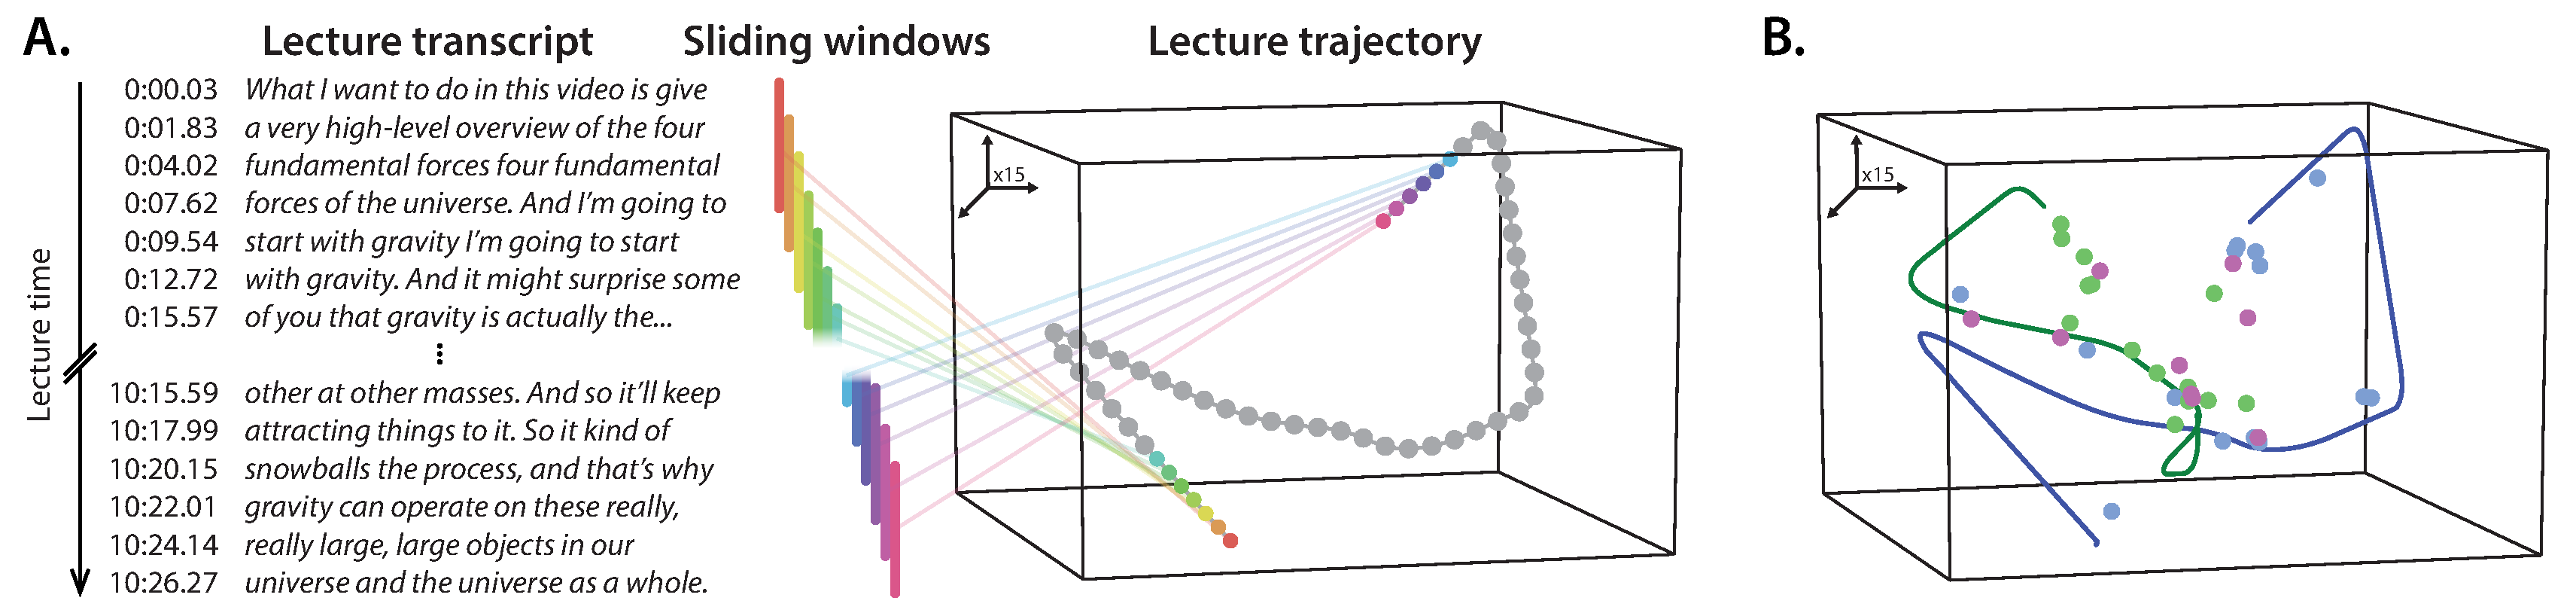
\includegraphics[width=\textwidth]{figs/sliding_windows}

    \caption{\textbf{Modeling course content.} \textbf{A. Building a document
    pool from sliding windows of text.} We decompose each lecture's transcript
    into a series of overlapping sliding windows. The full set of transcript
    snippets (across all windows) may be treated as a set of ``documents'' for
    training a text embedding model. \textbf{B. Constructing lecture content
    \textit{trajectories}.} After training the model on the sliding windows
    from both lectures, we transform each lecture into a ``trajectory'' through
    text embedding space by joining the embedding coordinates of successive
    sliding windows parsed from its transcript. \textbf{C. Embedding multiple
    lectures and questions in a shared space.} We apply the same model (trained
    on the two lectures' windows) to both lectures, along with the text of each
    question in our pool (Supp.~Tab.~\questions), to project them into a shared
    text embedding space. This results in one trajectory per lecture and one
    coordinate for each question. Here, we have projected the 15-dimensional
    embeddings onto their first 3 principal components for visualization.}

    \label{fig:sliding-windows}
\end{figure}

To study in detail how participants' conceptual knowledge changed over the
course of the experiment, we first sought to model the conceptual content
presented to them at each moment throughout each of the two lectures. We
adapted an approach we developed in prior work~\citep{HeusEtal21} to identify
the latent themes in the lectures using a topic model~\citep{BleiEtal03}.
Briefly, topic models take as input a collection of text documents, and learn a
set of ``topics'' (i.e., latent themes) from their contents. Once fit, a topic
model can be used to transform arbitrary (potentially new) documents into sets
of ``topic proportions,'' describing the weighted blend of learned topics
reflected in their texts. We parsed automatically generated transcripts of the
two lectures into overlapping sliding windows, where each window contained the
text of the lecture transcript from a particular time span. We treated the set
of text snippets (across all of these windows) as documents to fit the model
(Fig.~\ref{fig:sliding-windows}A; see~\nameref{subsec:topic-modeling}).
Transforming the text from every sliding window with the model yielded a
number-of-windows by number-of-topics (15) topic-proportions matrix describing
the unique mixture of broad themes from both lectures reflected in each
window's text. Each window's ``topic vector'' (i.e., column of the
topic-proportions matrix) is analogous to a coordinate in a 15-dimensional
space whose axes are topics discovered by the model. Within this space, each
lecture's sequence of topic vectors (i.e., corresponding to its transcript's
overlapping text snippets across sliding windows) forms a \textit{trajectory}
that captures how its conceptual content unfolds over time
(Fig.~\ref{fig:sliding-windows}B). We resampled these trajectories to a
resolution of one topic vector for each second of video (i.e., 1~Hz).

We hypothesized that a topic model trained on transcripts of the two lectures
should also capture the conceptual knowledge probed by each quiz question. If
indeed the topic model could capture information about the deeper conceptual
content of the lectures (i.e., beyond surface-level details such as particular
word choices), then we should be able to recover a correspondence between each
lecture and questions \textit{about} each lecture. Importantly, such a
correspondence could not solely arise from superficial text matching between
lecture transcripts and questions, since the lectures and questions often used
different words (Supp.~Fig.~\jaccard) and phrasings. Simply comparing the
average topic weights from each lecture and question set (averaging across time
and questions, respectively) reveals a striking correspondence 
(Supp.~Fig.~\topicWeights). Specifically, the average topic weights from Lecture~1 are
strongly correlated with the average topic weights from Lecture~1 questions
($r(13) = 0.809,~p < 0.001$, 95\% confidence interval (CI)~$= [0.633,~0.962]$),
and the average topic weights from Lecture~2 are strongly correlated with the
average topic weights from Lecture~2 questions ($r(13) = 0.728,~p = 0.002$,
95\% CI~$= [0.456,~0.920]$). At the same time, the average topic weights from
the two lectures are \textit{negatively} correlated with the average topic weights from their non-matching
question sets (Lecture~1 video vs.~Lecture~2 questions: $r(13) = -0.547,~p =
0.035$, 95\% CI~$= [-0.812, ~-0.231]$; Lecture~2 video vs.~Lecture~1 questions:
$r(13) = -0.612,~p = 0.015$, 95\% CI~$= [-0.874,~-0.281]$), indicating that the
topic model also exhibits some degree of specificity. The full set of pairwise
comparisons between average topic weights for the lectures and question sets is
reported in Supplementary Figure~\topicWeights.

\begin{figure}[tp]
    \centering
    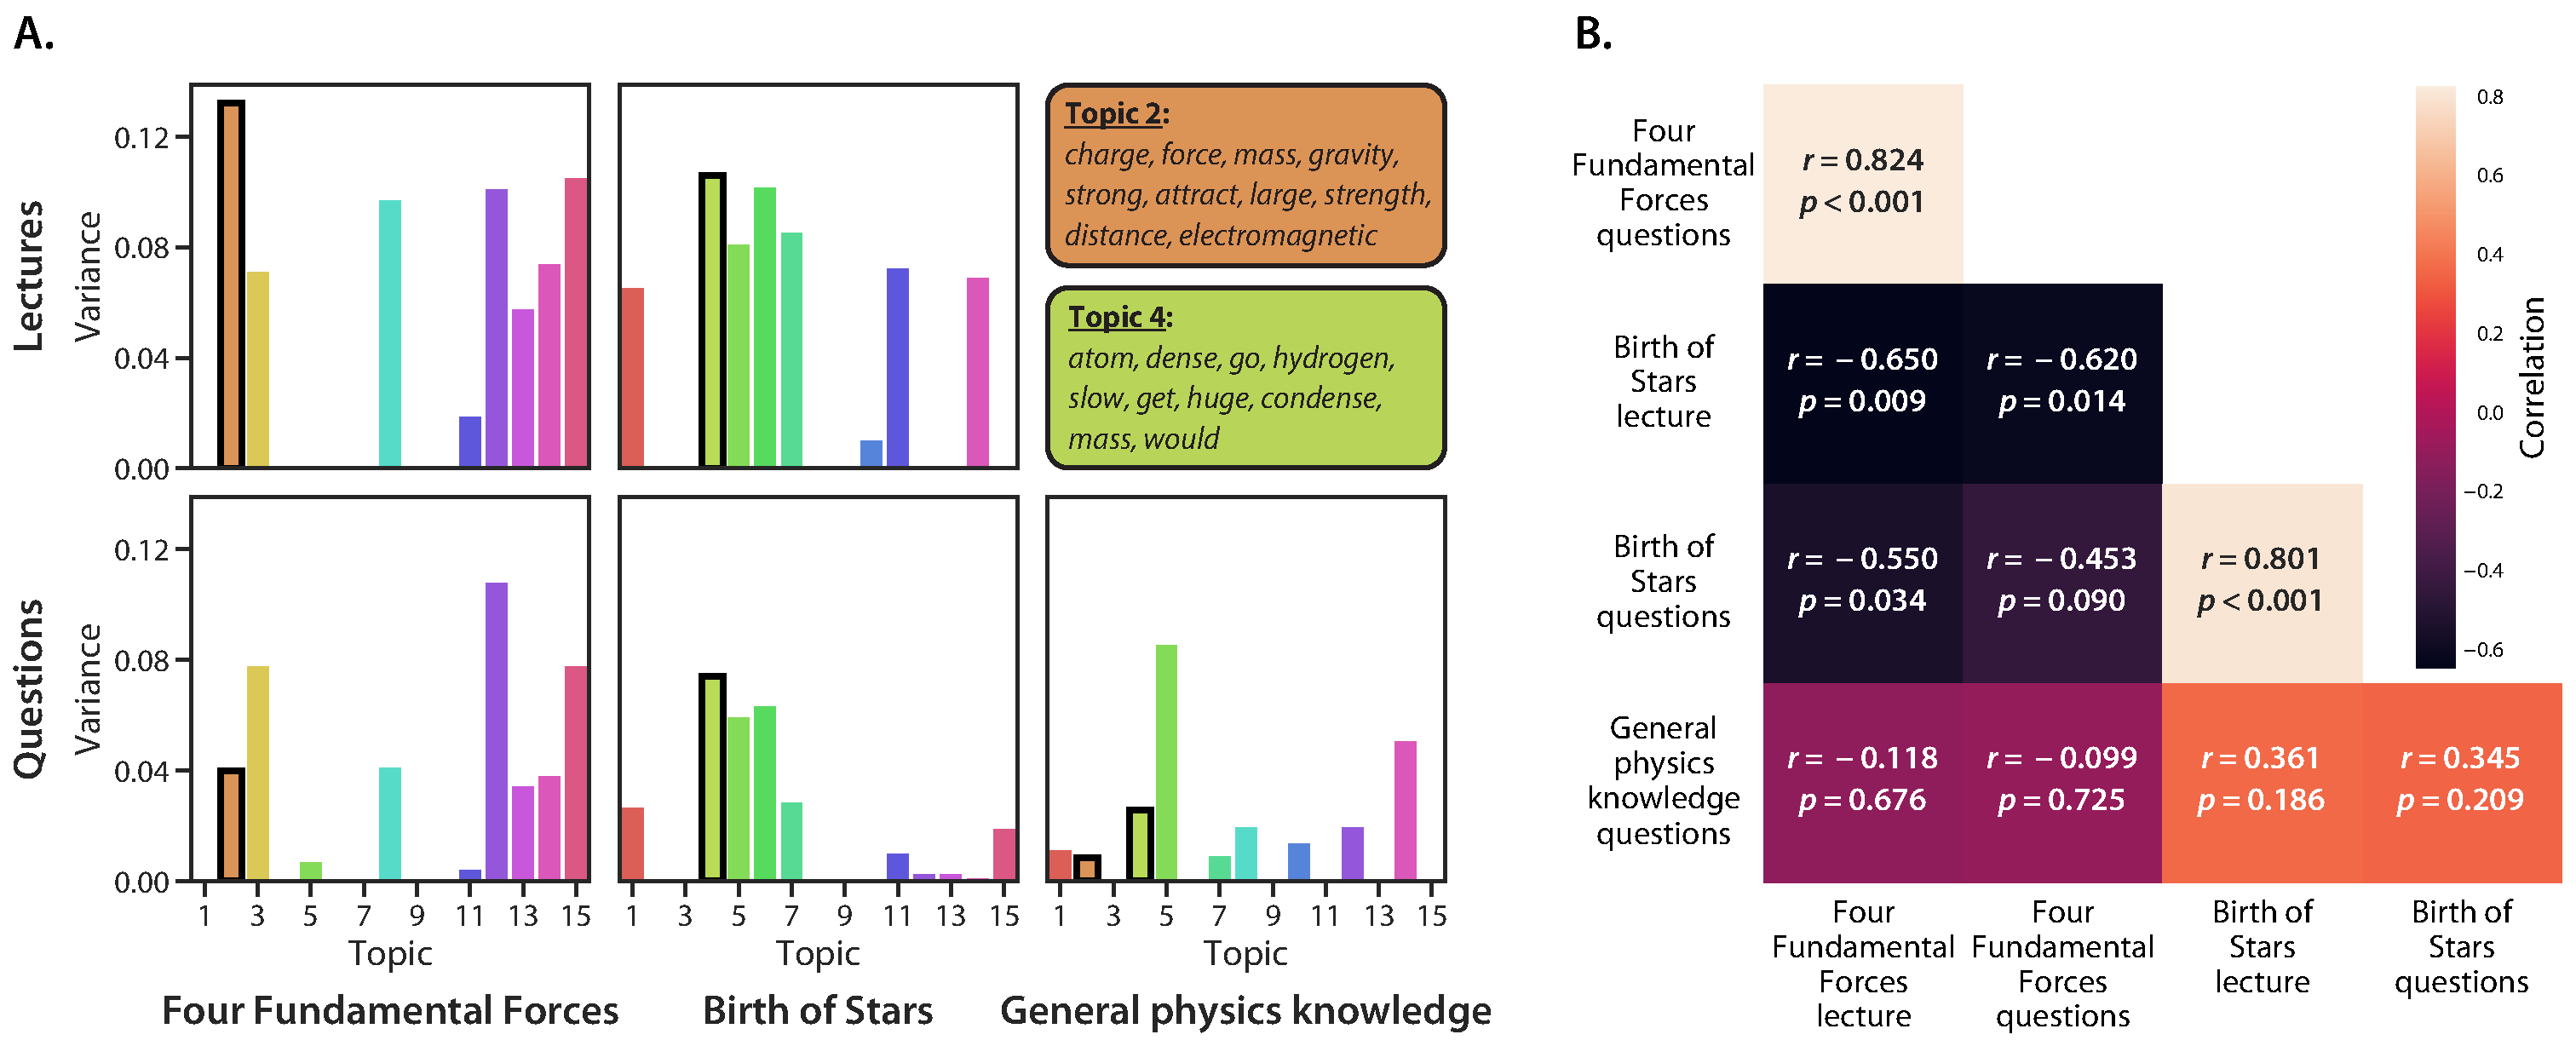
\includegraphics[width=\textwidth]{figs/active-topics}

    \caption{\textbf{Lecture and question topic overlap.} \textbf{A. Topic
    weight variability}. The bar plots display the variance of each topic's
    weight across lecture timepoints (top row) and questions (bottom row);
    colors denote topics. The top-weighted words from the most ``expressive''
    (i.e., variable across observations) topic from each lecture are displayed
    in the upper right (orange: topic 2; yellow-green: topic 4). The
    top-weighted words from the full set of topics may be found in
    Supplementary Table~\topics. \textbf{B. Relationships between topic weight
    variability.} Pairwise correlations between the distributions of topic
    weight variance for each lecture and question set. Each row and column
    corresponds to a bar plot in Panel A.}

    \label{fig:topics}
\end{figure}

Another, more sensitive, way of summarizing the conceptual content of the
lectures and questions is to look at \textit{variability} in how topics are
weighted over time and across different questions (Fig.~\ref{fig:topics}).
Intuitively, the variability in the expression of a given topic relates to how
much ``information''~\citep{Fish22} the lecture (or question set) reflects
about that topic. For example, suppose a given topic is weighted on heavily
throughout a lecture. That topic might be characteristic of some aspect or
property of the lecture \textit{overall} (conceptual or otherwise), but unless
the topic's weights changed in meaningful ways over time, the topic would be a
poor indicator of any \textit{specific} conceptual content in the lecture. We
therefore also compared the variances in topic weights (across time or
questions) between the lectures and questions. The variability in topic
expression (over time and across questions) was similar for the Lecture~1 video
and questions ($r(13) = 0.824,~p<0.001$, 95\% CI~$= [0.696,~0.973]$) and the
Lecture~2 video and questions ($r(13) = 0.801,~p<0.001$, 95\% CI~$=
[0.539,~0.958]$). Simultaneously, as reported in Figure~\ref{fig:topics}B, the
variabilities in topic expression across \textit{different} videos and
lecture-specific questions (i.e., Lecture~1 video vs.~Lecture~2 questions;
Lecture~2 video vs.~Lecture~1 questions) were negatively correlated, and
neither video's topic variability was reliably correlated with the topic
variability across general physics knowledge questions. Taken together, the
analyses reported in Figure~\ref{fig:topics} and Supplementary
Figure~\topicWeights~indicate that a topic model fit to the videos' transcripts
can also reveal correspondences (at a coarse scale) between the lectures and
questions.

While an individual lecture may be organized around a single broad theme at a
coarse scale, at a finer scale, each moment of a lecture typically covers a
narrower range of content. Given the correspondence we found between the
variabilities in topic expression across moments of each lecture and questions
from its corresponding set (Fig.~\ref{fig:topics}), we wondered whether the
text embedding model might additionally capture these conceptual relationships
at a finer scale. For example, if a particular question asks about the content
from one small part of a lecture, we wondered whether the text embeddings could
be used to automatically identify the ``matching'' moment(s) in the lecture. To
explore this, we computed the correlation between each question's topic weights
and the topic weights for each second of its corresponding lecture, and found
that each question appeared to be temporally specific
(Fig.~\ref{fig:question-correlations}). In particular, most questions' topic
vectors were maximally correlated with a well-defined (and relatively narrow)
range of timepoints from their corresponding lectures, and the correlations
fell off sharply outside of that range (Supp.~Figs.~\forcesCorrs,~\bosCorrs).
We also qualitatively examined the best-matching intervals for each question by
comparing the question's text to the transcribed text from the most-correlated parts of the
lectures (Supp.~Tab.~\matchTab). Despite that the questions were excluded from
the text embedding model's training set, in general we found (through manual
inspection) a close correspondence between the conceptual content that each
question probed and the content covered by the best-matching moments of the
lectures. Two representative examples are shown at the bottom of
Figure~\ref{fig:question-correlations}.

\begin{figure}[t]
    \centering
    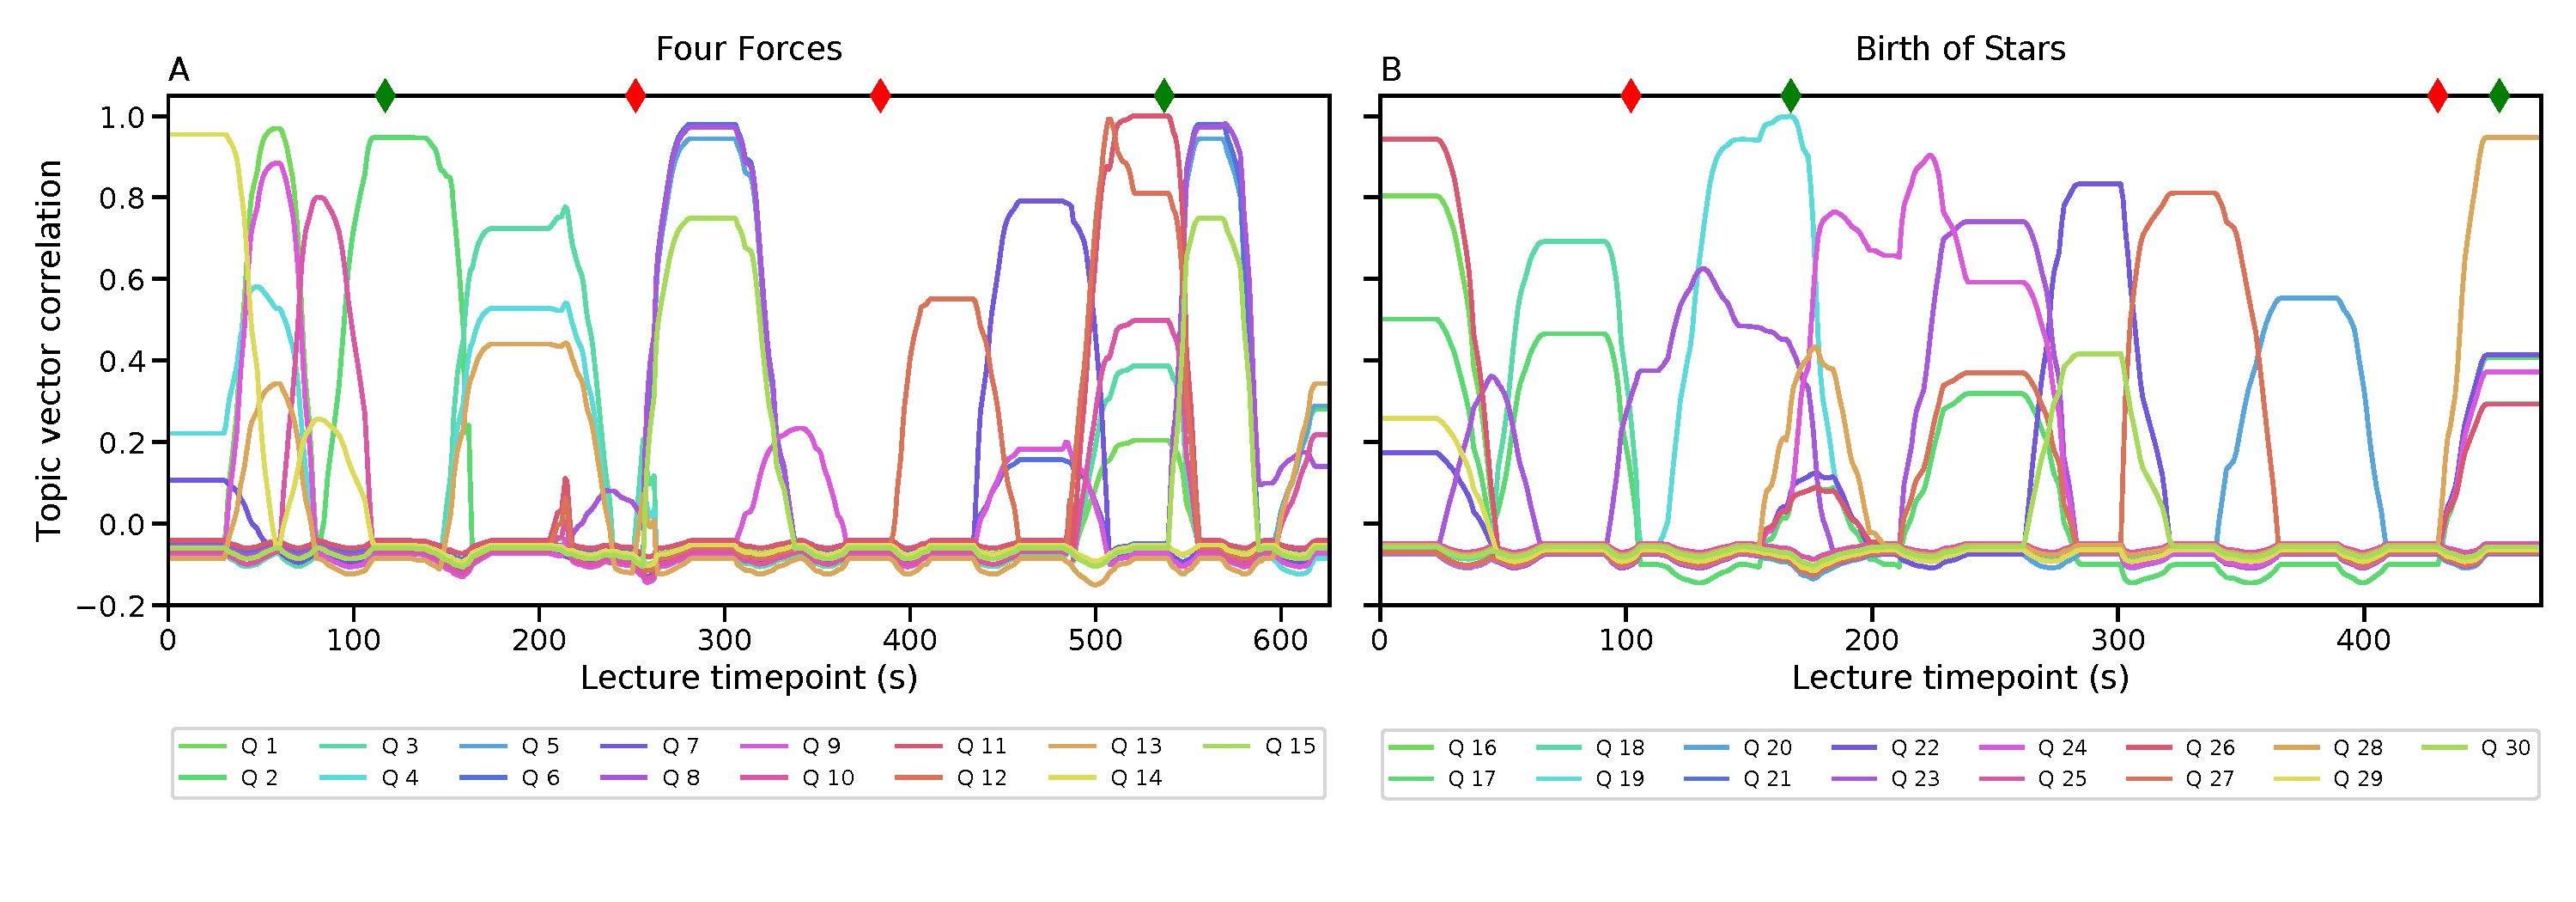
\includegraphics[width=\textwidth]{figs/lecture-question-similarity}

    \caption{\textbf{Which parts of each lecture are captured by each
    question?} Each panel displays time series plots showing how each question's
    topic vector correlates with each video timepoint's topic vector (Panel
    \textbf{A.}: correlations for the \textit{Four Fundamental Forces} lecture
    and associated questions; Panel \textbf{B.}: correlations for the
    \textit{Birth of Stars} lecture and associated questions). The colors
    denote question identities. The diamonds in each panel denote the moment of
    peak correlation between the indicated question and the lecture trajectory.
    The associated questions' text and snippets of the lectures' transcripts
    from the surrounding 30 seconds, are displayed at the bottom of the
    figure.}

    \label{fig:question-correlations}
\end{figure}

The ability to quantify how much each question is ``asking about'' the content
from each moment of the lectures could enable high-resolution insights into
participants' knowledge. Traditional approaches to estimating how much a
student ``knows'' about the content of a given lecture entail administering some form of assessment (e.g., a quiz) and computing the
proportion of correctly answered questions. But if two students receive
identical scores on such an exam, might our modeling framework help us to gain more
nuanced insights into the \textit{specific} content that each student has
mastered (or failed to master)? For example, a student who misses three
questions that were all about the same concept (e.g., concept $A$) will have
gotten the same \textit{proportion} of questions correct as another student who
missed three questions about three \textit{different} concepts (e.g., $A$, $B$,
and $C$). But if we wanted to help these two students fill in the ``gaps'' in
their understandings, we might do well to focus specifically on concept $A$ for
the first student, but to also add in materials pertaining to concepts $B$ and
$C$ for the second student. In other words, raw ``proportion-correct'' measures
may capture \textit{how much} a student knows, but not \textit{what} they know.
We wondered whether our modeling framework might enable us to (formally and
automatically) infer participants' knowledge at the scale of individual
concepts (e.g., as captured by a single moment of a lecture).

We developed a simple formula (Eqn.~\ref{eqn:prop}) for using a participant's
responses to a small set of multiple-choice questions to estimate how much the
participant ``knows'' about the concept reflected by any arbitrary coordinate
$x$ in text embedding space (e.g., the content reflected by any moment in a
lecture they had watched; see \nameref{subsec:traces}). Essentially, the
estimated knowledge at coordinate $x$ is given by the weighted
proportion of quiz questions the participant answered correctly, where the
weights reflect how much each question is ``about'' the content at $x$. When we
apply this approach to estimate the participant's knowledge about the content
presented in each moment of each lecture, we can obtain a detailed time course
describing how much ``knowledge'' that participant has about the content
presented at any part of the lecture. As shown in
Figure~\ref{fig:knowledge-timeseries}A and C, we can apply this approach
separately for the questions from each quiz participants took throughout the
experiment. From just a few questions per quiz (see~\nameref{subsec:traces}),
we obtain a high-resolution snapshot (at the time each quiz was taken) of what
the participants knew about any moment's content, from either of the two
lectures they watched (comprising a total of 1,100 samples across the two
lectures).

\begin{figure}[tp]
    \centering
    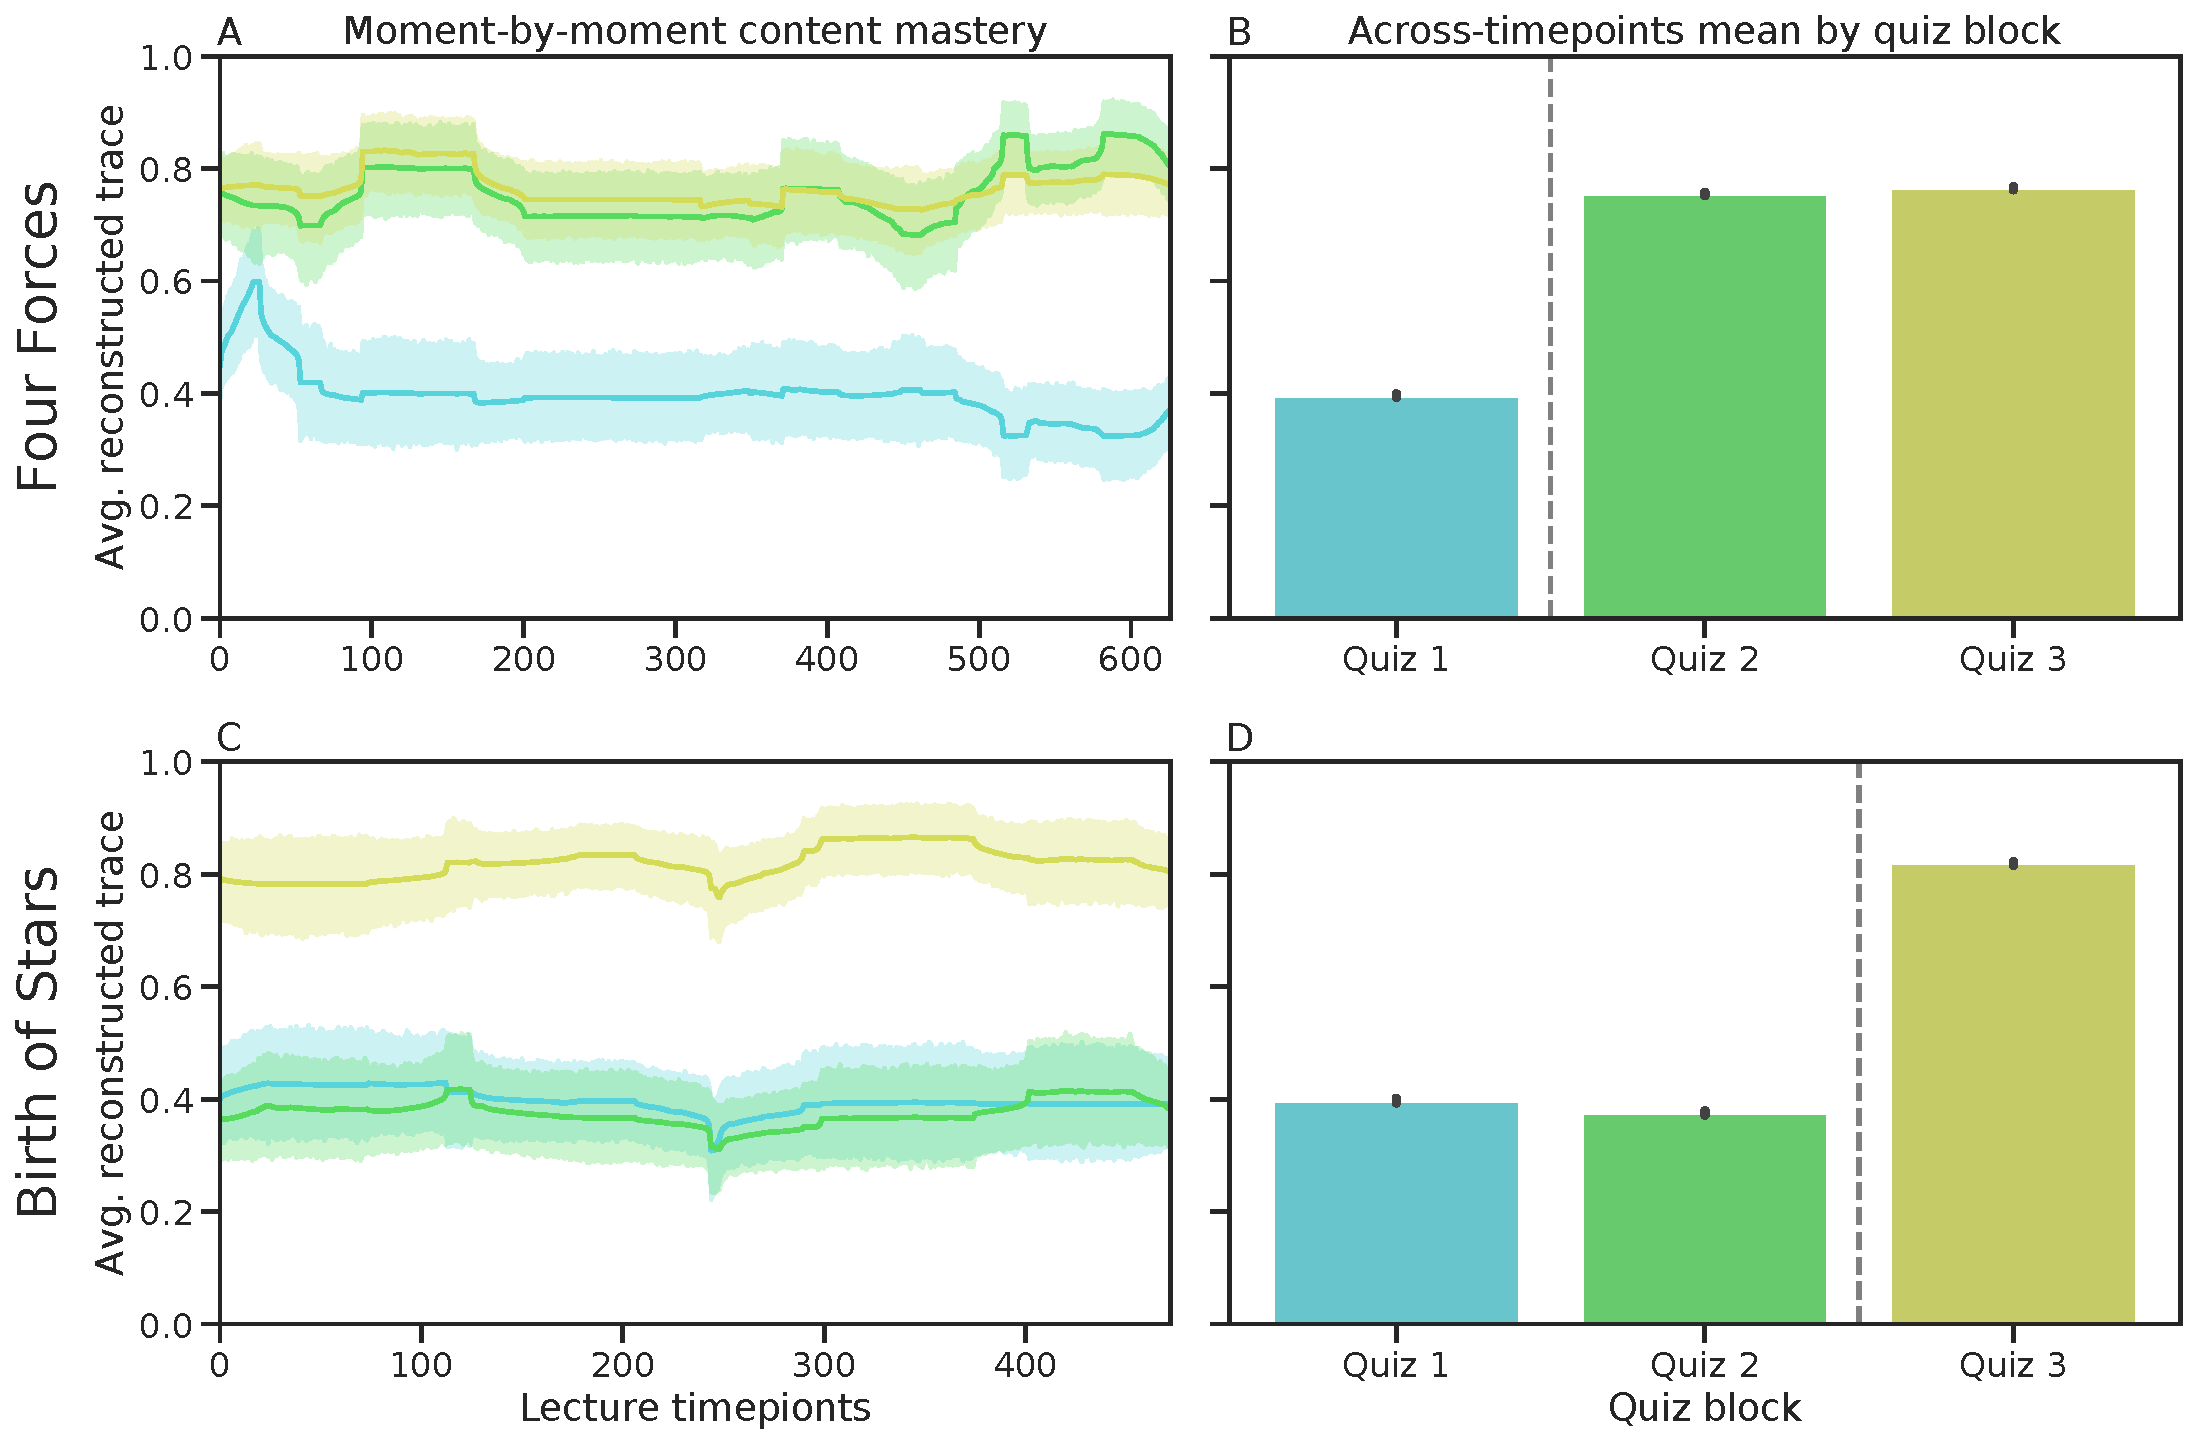
\includegraphics[width=0.7\textwidth]{figs/content-mastery}

    \caption{\textbf{Estimating knowledge about the content presented at each
    moment of each lecture.} \textbf{A. Knowledge about the time-varying
    content of \textit{Four Fundamental Forces}}. Each trace displays the
    weighted proportion of correctly answered questions about the content
    reflected in each moment of the lecture (see \nameref{subsec:traces}),
    using responses from a single quiz (color). The traces are averaged across
    participants. \textbf{B. Average estimated knowledge about \textit{Four
    Fundamental Forces}.} Each bar displays the across-timepoint average
    knowledge, estimated using the responses to one quiz's questions.
    \textbf{C. Knowledge about the time-varying content of \textit{Birth of
    Stars}}. The panel is in the same format as Panel A, but here the knowledge
    estimates are for the moment-by-moment content of the \textit{Birth of
    Stars} lecture. \textbf{D. Average estimated knowledge about \textit{Birth
    of Stars}.} The panel is in the same format as Panel B, but here the
    knowledge estimates are for the content of the \textit{Birth of Stars}
    lecture. All panels: error ribbons and error bars denote 95\% confidence
    intervals, estimated across participants.}

    \label{fig:knowledge-timeseries}
\end{figure}

While the time courses in Figure~\ref{fig:knowledge-timeseries}A and C provide
detailed \textit{estimates} about participants' knowlege, these estimates are
of course only \textit{useful} to the extent that they accurately reflect what
participants actually know. As one sanity check, we anticipated that the
knowledge estimates should reflect a content-specific ``boost'' in
participants' knowledge after watching each lecture. In other words, if
participants learn about each lecture's content upon watching it,
the knowledge estimates should capture that. After watching the \textit{Four
Fundamental Forces} lecture, participants should exhibit more knowledge for the
content of that lecture than they had before, and that knowledge should persist
for the remainder of the experiment. Specifically, knowledge about that
lecture's content should be relatively low when estimated using Quiz~1
responses, but should increase when estimated using Quiz~2 or 3 responses
(Fig.~\ref{fig:knowledge-timeseries}B). Indeed, we found that participants'
estimated knowledge about the content of \textit{Four Fundamental Forces}
was substantially higher on Quiz~2 versus Quiz~1 ($t(49) = 8.764,~p < 0.001$)
and on Quiz~3 versus Quiz~1 ($t(49) = 10.519,~p < 0.001$). We found no reliable
differences in estimated knowledge about that lecture's content on Quiz~2
versus 3 ($t(49) = 0.160,~p = 0.874$). Similarly, we hypothesized (and
subsequently confirmed) that participants should show greater estimated
knowledge about the content of the \textit{Birth of Stars} lecture after
(versus before) watching it (Fig.~\ref{fig:knowledge-timeseries}D).
Specifically, since participants watched that lecture after taking Quiz~2 (but
before Quiz~3), we hypothesized that their knowledge estimates should be
relatively low on Quizzes~1 and 2, but should show a ``boost'' on Quiz~3.
Consistent with this prediction, we found no reliable differences in estimated
knowledge about the \textit{Birth of Stars} lecture content on Quizzes~1 versus
2 ($t(49) = 1.013,~p = 0.316$), but the estimated knowledge was substantially
higher on Quiz~3 versus 2 ($t(49) = 10.561,~p < 0.001$) and Quiz~3 versus 1
($t(49) = 8.969,~p < 0.001$).

If we are able to accurately estimate a participant's knowledge about the
content tested by a given question, our estimates of their knowledge should
carry some predictive information about whether they are likely to answer that 
question correctly or incorrectly. We developed a statistical approach to test this claim. 
For each quiz question a participant answered, in turn, we used Equation~\ref{eqn:prop} to estimate their knowledge at the given question's embedding space coordinate based on other questions that participant answered on the same quiz. 
We repeated this for all participants, and for each of the three quizzes. 
Then, separately for each quiz, we fit a generalized linear mixed model (GLMM) with a logistic link function to explain the likelihood of correctly answering a question as a function of estimated knowledge for its embedding coordinate, while accounting for random variation among participants and questions (see \nameref{subsec:glmm}).
To assess the predictive value of the knowledge estimates, we compared each GLMMs to an analogous (i.e., nested) ``null'' model that did not consider estimated knowledge using parametric bootstrap likelihood-ratio tests.

\begin{figure}[tp]
    \centering
    % TODO: adjust width to max possible based on finalized caption
    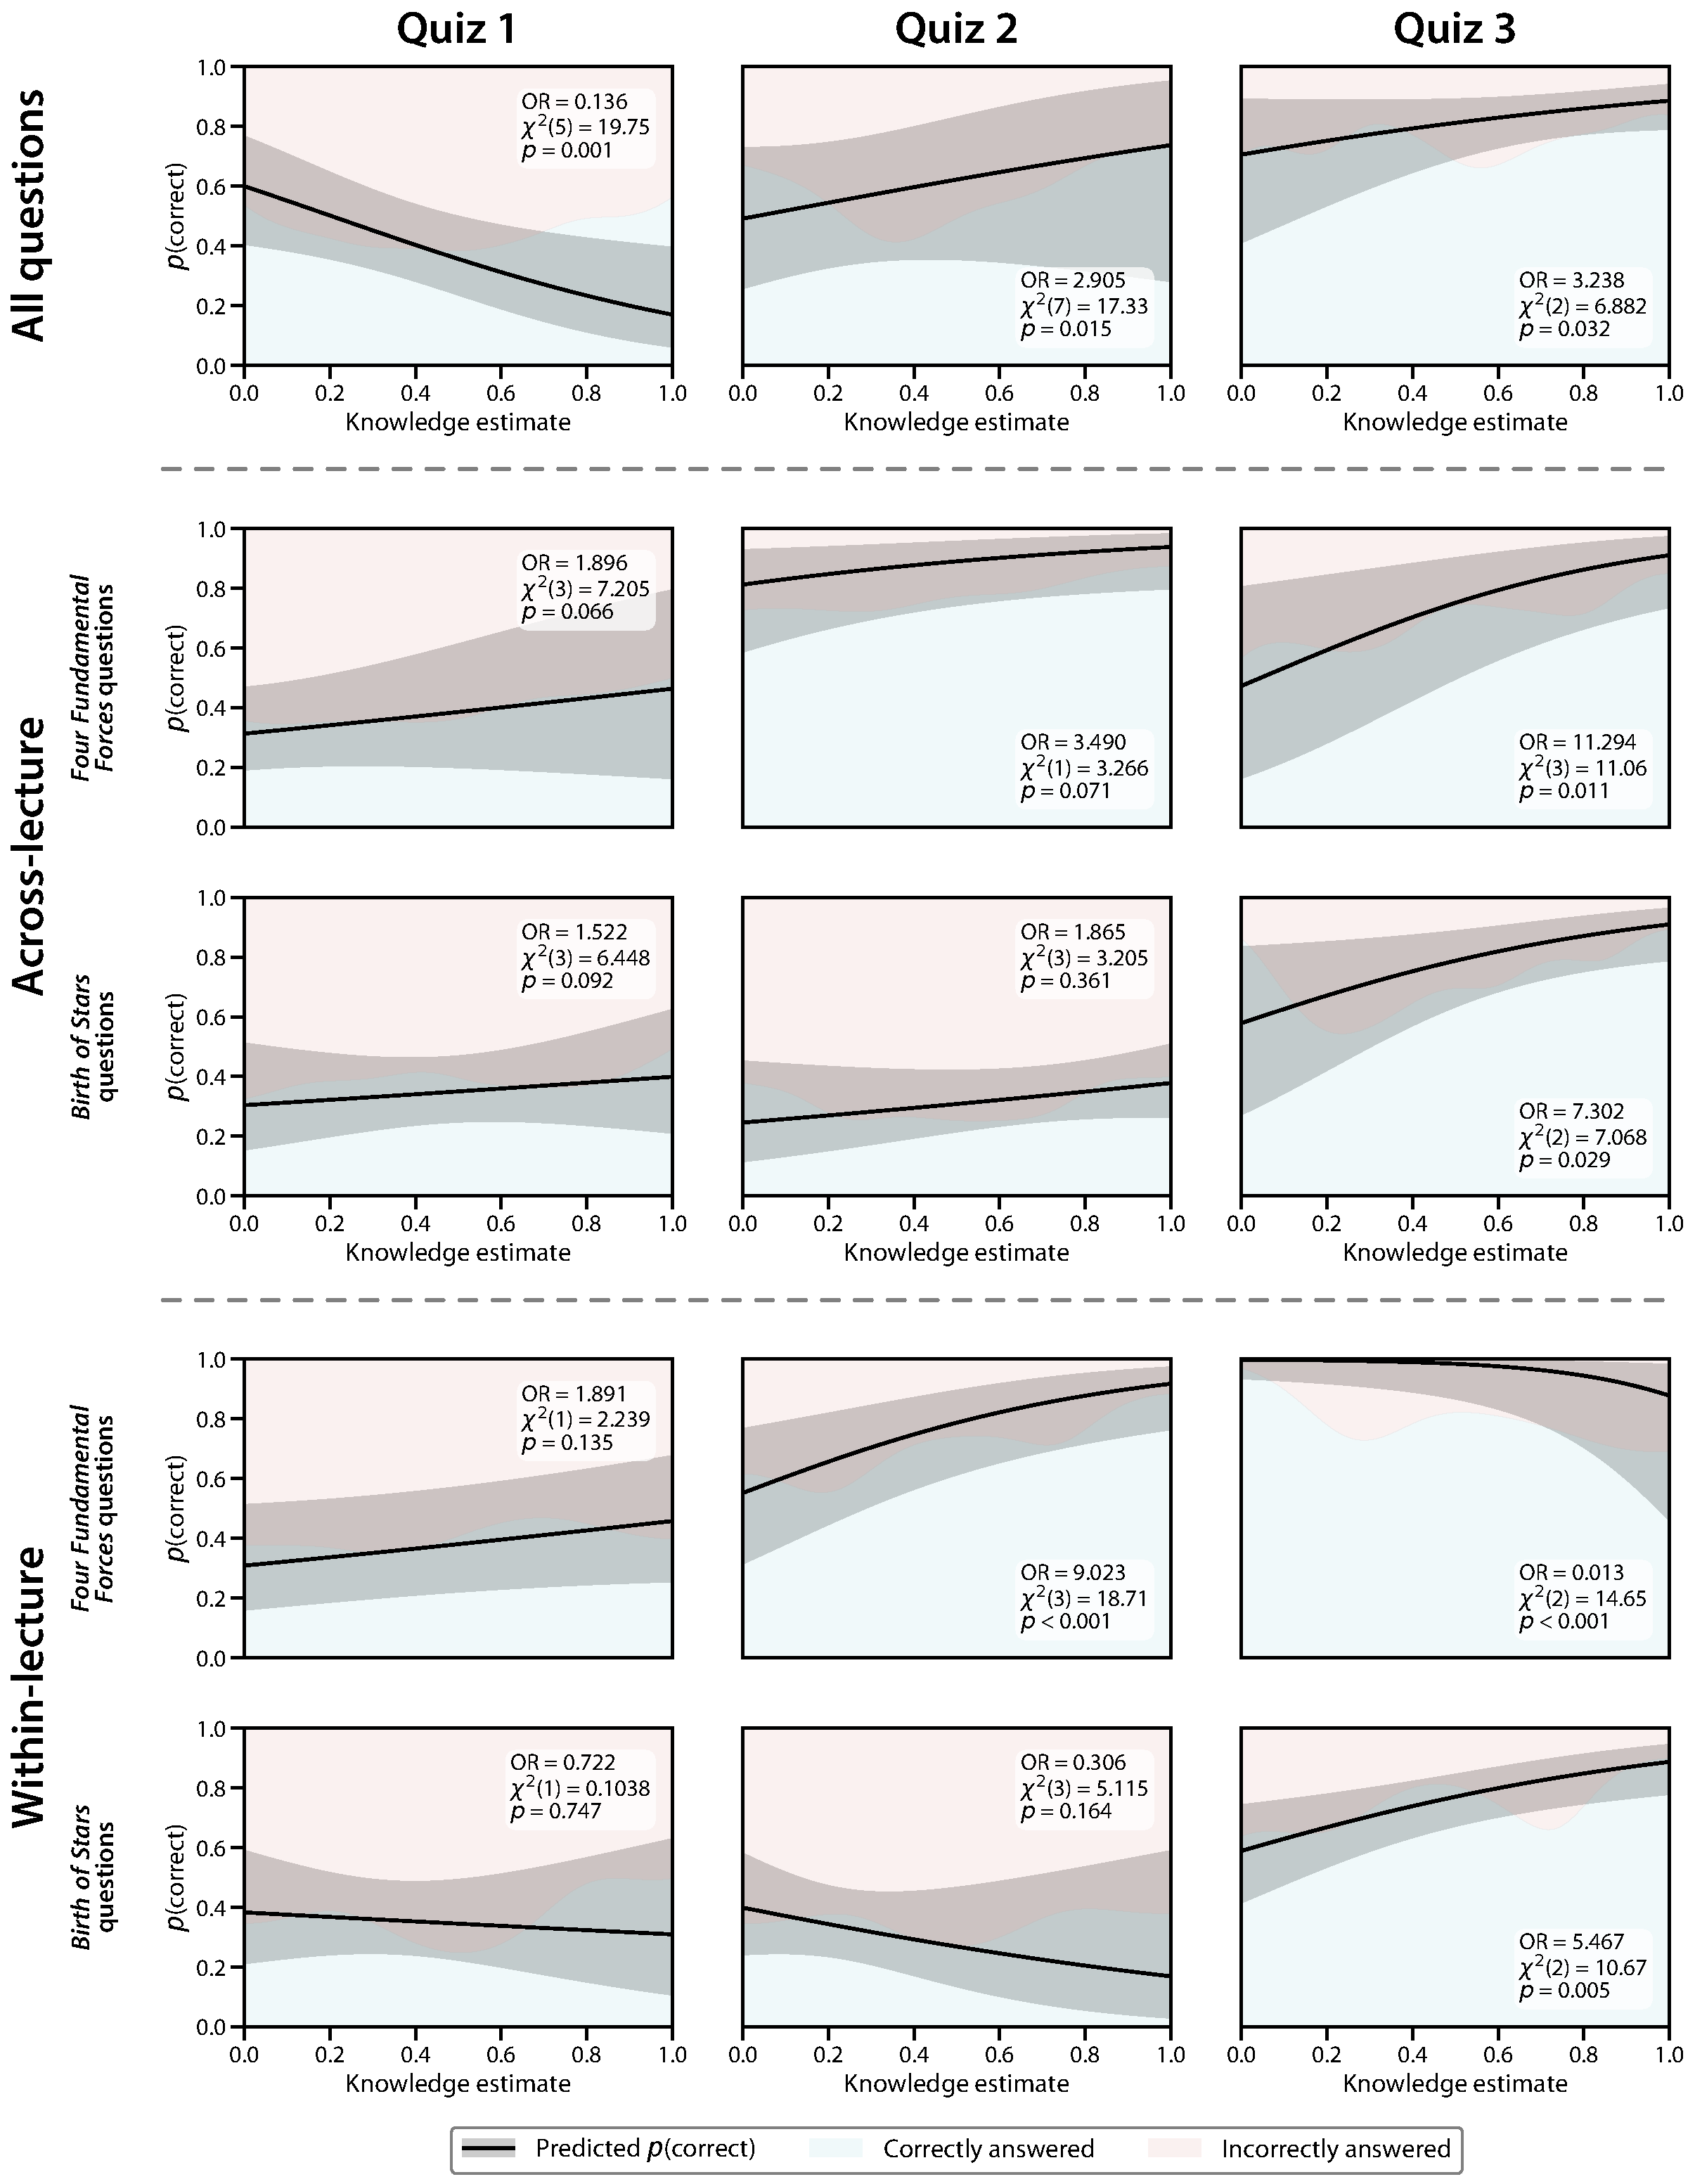
\includegraphics[width=0.7\textwidth]{figs/predict-knowledge-questions}
    \caption{\textbf{Predicting success on held-out questions using estimated knowledge.}
    We used generalized linear mixed models (GLMMs) to model the likelihood of correctly answering a quiz question as a function of estimated knowledge for its embedding coordinate (see \nameref{subsec:glmm}). 
    Separately for each quiz (column), we examined this relationship based on three different sets of knowledge estimates: knowledge for each question based on all other questions the same participant answered on the same quiz (``All questions''; top row), knowledge for each question about one lecture based on all questions (from the same participant and quiz) about the \textit{other} lecture (``Across-lecture''; middle rows), and knowledge for each question about one lecture based on all other questions (from the same participant and quiz) about the \textit{same} lecture (``Within-lecture''; bottom rows). 
    The background in each panel displays the relative density of observed correctly (blue) versus incorrectly (red) answered questions over the range of knowledge estimates. 
    The black curves display the (population-level) GLMM-predicted probabilities of correctly answering a question as a function of estimated knowledge. 
    Error ribbons denote 95\% confidence intervals.}

    \label{fig:predictions}
\end{figure}

We carried out three different versions of the analyses described above, wherein we considered different sources of information in our estimates of participants' knowledge for each quiz question. 
First, we estimated knowledge at each question's embedding coordinate using \textit{all other} questions answered by the same participant on the same quiz (``All questions''; Fig.~\ref{fig:predictions}, top row).
This test was intended to assess the overall predictive power of our approach. 
Second, we estimated knowledge for each question about one lecture using only questions (from the same participant and quiz) about the \textit{other} lecture (``Across-lecture''; Fig.~\ref{fig:predictions}, middle rows). 
This test was intended to assess the \textit{generalizability} of our approach by asking whether our predictions held across the content areas of the two lectures.
Third, we estimated knowledge for each question about a given lecture using only the other questions (from the same participant and quiz) about that \textit{same} lecture (``Within-lecture''; Fig.~\ref{fig:predictions}, bottom rows). 
This test was intended to assess the \textit{specificity} of our approach by asking whether our predictions could distinguish between questions about different content covered by the same lecture.

%When we estimated participants' knowledge for each Quiz~1 question based on all other Quiz~1 questions, we found an inverse relationship. 
%Specifically, higher estimated knowledge at the embedding coordinate at a held-out question was associated with a lower likelihood of answering the question correctly ($\textrm{odds ratio}\ (OR) = 0.136,\ \textrm{likelihood-ratio test statistic}\ (\lambda_{LR}) = 19.749,\ \textrm{95\% CI} = [14.352,\ 26.545],\ p = 0.001$). 
%However, this inverse relationship in fact represents the expected result under our null hypothesis (that estimated knowledge is \textit{not} predictive of success on a question). 
%An intuition for this can be taken from the expected outcome of same analysis based on the simple proportion correct, rather than estimated knowledge. 
%Suppose a participant answered $n$ out of 13 quiz questions correctly. 
%If we held out a single correctly answered question and computed the proportion of remaining questions answered correctly, that proportion would be $(n - 1) / 12$. 
%Whereas if we held out a single incorrectly answered question, the proportion of remaining questions answered correctly would be $n / 12$. 

In performing this set of analyses, our null hypothesis is that the knowledge estimates we compute based on the quiz questions' embedding coordinates do \textit{not} provide useful information about participants' abilities to answer those questions. 
What result might we expect to see if this is the case? 
To provide an intuition for this, consider the expected outcome if we carried out these same analyses using a simple proportion-correct measure in lieu of our knowledge estimates. 
Suppose a participant correctly answered $n$ out of 13 questions on a given quiz. 
If we held out a single correctly answered question and computed the proportion of remaining questions answered correctly, that proportion would be $(n - 1) / 12$. 
Whereas if we held out a single \textit{incorrectly} answered question and did the same, that proportion would be $n / 12$. 
Thus for a given participant and quiz, a ``knowledge estimate'' computed as the simple (i.e., unweighted) remaining proportion-correct is perfectly inversely related to success on a held-out question: it will always be \textit{lower} for correctly answered questions than for incorrectly answered questions. 
Given that our knowledge estimates are computed as a weighted version of this same proportion-correct score (where each held-in question's weight reflects its embedding-space distance from the held-out question; see Eqn.~\ref{eqn:prop}), if these weights are uninformative (e.g., simply randomly distributed), then we should expect to see this same inverse relationship emerge, on average. 
It is only if the spatial relationships among the quiz questions' embedding coordinates map onto participants' knowledge in a meaningful way that we would we expect this relationship to be non-negative [\textbf{PHRASING}].

When we fit a GLMM to estimates of participants' knowledge for each Quiz~1 question based on all other Quiz~1 questions, we observed this null-hypothesized inverse relationship. 
Specifically, higher estimated knowledge at the embedding coordinate of a held-out Quiz~1 question was associated with a lower likelihood of answering the question correctly (odds ratio $(OR) = 0.136$, likelihood-ratio test statistic $(\lambda_{LR}) = 19.749$, 95\%\ $\textnormal{CI} = [14.352,\ 26.545],\ p = 0.001$). 
However, when we repeated this analysis for quizzes 2 and 3, the direction of this relationship reversed: higher estimated knowledge for a given question predicted a greater likelihood of answering it correctly (Quiz~2: $OR = 2.905,\ \lambda_{LR} = 17.333,\ 95\%\ \textnormal{CI} = [14.966,\ 29.309],\ p = 0.002$; Quiz~3: $OR = 3.238,\ \lambda_{LR} = 6.882,\ 95\%\ \textnormal{CI} = [6.228,\ 8.184],\ p = 0.017$). 
Taken together, these results suggest that our knowledge estimations can reliably predict participants' likelihood of success on individual quiz questions, provided they have at least some amount of structured knowledge about the underlying concepts being tested. 
In other words, when participants' correct responses primarily arise from knowledge about the content probed by each question (e.g., after watching one or both lectures), these successes can be predicted from their ability to answer other questions about conceptually similar content (as captured by embedding-space distance).
However, when a sufficiently large portion of participants' correct responses (presumably) reflect successful random guessing (such as on a multiple-choice quiz taken before viewing either lecture), our approach fails to accurately predict these successes since they do not map onto embedding space distances in a meaningful way [\textbf{PHRASING}].

We observed a similar pattern when we fit GLMMs to estimates of participants' knowledge for each question about one lecture derived from other questions about the \textit{same} lecture. 
Specifically, for questions that participants answered on Quiz~1, prior to watching either lecture, knowledge for the embedding coordinates of \textit{Four Fundamental Forces}-related questions estimated using other \textit{Four Fundamental Forces}-related questions did not reliably predict whether those questions were answered correctly ($OR = 1.891,\ \lambda_{LR} = 2.293,\ 95\%\ \textnormal{CI} = [2.091,\ 2.622],\ p = 0.139$). 
The same was true of knowledge estimates for \textit{Birth of Stars}-related questions based on other \textit{Birth of Stars}-related questions ($OR = 0.722,\ \lambda_{LR} = 5.115,\ 95\%\ \textnormal{CI} = [0.094,\ 0.146],\ p = 0.738$). 
When we recomputed these within-lecture knowledge estimates using questions from Quiz~2---which participants took immediately after viewing \textit{Four Fundamental Forces} but prior to viewing \textit{Birth of Stars}---we found that they now reliably predicted success on \textit{Four Fundamental Forces}-related questions ($OR = 9.023,\ \lambda_{LR} = 18.707,\ 95\%\ \textnormal{CI} = [10.877,\ 22.222],\ p = 0.001$) but not on \textit{Birth of Stars}-related questions ($OR = 0.306,\ \lambda_{LR} = 5.115,\ 95\%\ \textnormal{CI} = [4.624,\ 5.655],\ p = 0.055$).
Using participants' responses from Quiz~3 (taken immediately after viewing \textit{Birth of Stars}), we found that within-lecture knowledge estimates for \textit{Birth of Stars}-related questions could now reliably predict success on those questions ($OR = 5.467,\ \lambda_{LR} = 10.670,\ 95\%\ \textnormal{CI} = [7.998, 12.532],\ p = 0.006$). 
However, within-lecture knowledge estimates for \textit{Four Fundamental Forces} questions answered on Quiz~3 were no longer directly related to the likelihood of successfully answering them and instead exhibited the inverse relationship we would expect to arise from unstructured knowledge (with respect to the embedding space; $OR = 0.013,\ \lambda_{LR} = 14.648,\ 95\%\ \textnormal{CI} = [10.695, 23.096],\ p = 0.001$).
Speculatively, we suggest that this may reflect participants forgetting some of the \textit{Four Fundamental Forces} content (e.g., perhaps in favor of prioritizing encoding the just-watched \textit{Birth of Stars} content in preparation for the third quiz). 
If this forgetting happens in a relatively ``random'' way (with respect to spatial distance within the embedding space), then it could explain why some held-out questions about \textit{Four Fundamental Forces} were answered incorrectly, even if questions at nearby coordinates (i.e., about similar content) were answered correctly.
This might lead our approach to over-estimate knowledge for held-out questions about ``forgotten'' knowledge that participants answered incorrectly.
% ALTERNATE EXPLANATION -- embedding space is essentially ``saturated'' with correctly answered questions, so just like how on quiz 1 when relatively few questions are correct, most questions ``around'' them will be incorrect, on quiz 3 when relatively few questions are incorrect, most questions nearby will be correct. And because of this, on average, when the ``held-out'' question is one of the few incorrect ones, there will tend to be more correct ones ``held in'' than there will be when the held-out question is correct.
% Also, maybe worth noting: while negative relationship is significant, it's super weak -- per the model, a "1-unit" increase in estimated knowledge corresponds to only a 1.28% decrease in probability of correct answer (p = OR / (1 + OR)). For comparison, for quiz3/within-lecture/birth of stars, 1-unit increase in estimated knowledge corresponds to a 84.5% increase in probability. So decrease is sig. but basically negligible.
Taken together, these results suggest that our approach can distinguish between questions about different content covered by a single lecture when participants have sufficiently structured knowledge about that lecture's content, though this specificity may decrease further in time from when the lecture in question was viewed.

Finally, when we fit GLMMs to estimates of participants' knowledge for questions about one lecture based on questions (from the same quiz) about the other lecture, we observed a similar but slightly more nuanced pattern. 
Essentially, while the previous set of analyses suggest that our approach's ability to make \textit{specific} predictions within content areas depends on participants having a minimum level of knowledge about the given content, the across-lecture analyses we performed suggest that our ability to \textit{generalize} these predictions across different content areas requires that participants' level of knowledge about the content used to make predictions be reasonably similar to their level of knowledge about the content for which these predictions are made [\textbf{PHRASING}].
We found that using questions answered on Quiz~1, participants abilities to correctly answer questions about \textit{Four Fundamental Forces} could be predicted from their responses to questions about \textit{Birth of Stars} ($OR = 1.896,\ \lambda_{LR} = 7.205,\ 95\%\ \textnormal{CI} = [6.224, 7.524],\ p = 0.039$) and their ability to correctly answer \textit{Birth of Stars}-related questions could be predicted from their responses to \textit{Four Fundamental Forces}-related questions ($OR = 1.522,\ \lambda_{LR} =  6.448,\ 95\%\ \textnormal{CI} = [5.656, 6.843],\ p = 0.043$).
We note, however, that these Quiz~1 knowledge estimates suffer from the same ``noise'' due to the (presumably) higher rate of participants successfully guessing correct answers on Quiz~1 as noted above, and as a result provide the weakest signal of any of the knowledge estimates that we found to reliably predict success.
When we repeated this analysis using questions from Quiz~2, we found participants' responses to \textit{Four Fundamental Forces}-related questions did not reliably predict their success on \textit{Birth of Stars}-related questions ($OR = 1.865,\ \lambda_{LR} = 3.205,\ 95\%\ \textnormal{CI} = [3.027, 3.600],\ p = 0.125$), nor did their responses to \textit{Birth of Stars}-related questions reliably predict their success on \textit{Four Fundamental Forces}-related questions ($OR = 3.490,\ \lambda_{LR} = 3.266,\ 95\%\ \textnormal{CI} = [3.033, 3.866],\ p = 0.094$). 
\textbf{Sentence about why this makes sense given that participants hadn't viewed BoS yet. i.e., when predicting held-out FFF questions, correct vs. incorrect labels for held-in q's aren't meaningfully structured w.r.t. embedding space; when predicting held-out BoS q's, whether or not held-out q was correctly answered isn't meaningfully related to spatial structure of correctly answered q's in embedding space.}
However, when we again computed these across-lecture knowledge predictions using questions from Quiz~3 (when participants had now viewed \textit{both} lectures, we found that we could again reliably predict success on questions about \textit{Four Fundamental Forces} ($OR = 11.294),\ \lambda_{LR} = 11.055,\ 95\%\ \textnormal{CI} = [9.126, 18.476],\ p = 0.004$) and \textit{Birth of Stars} ($OR = 7.302),\ \lambda_{LR} = 7.068,\ 95\%\ \textnormal{CI} = [6.490, 8.584],\ p = 0.017$).
Across all three versions of these analyses, our results suggest that our knowledge estimations can reliably predict participants' abilities to answer individual quiz questions, distinguish between questions about similar content, and generalize across content areas, provided that participants' quiz responses reflect a minimum level of ``real'' knowledge about both content on which these predictions are based and that for which they are made [\textbf{PHRASING}].

% our approach works when participants have a minimal baseline level of knowledge about content predicted and used to predict
% our approach generalizes when knowledge of content used to predict can be assumed to be a reasonable indicator of knowledge of content predicted
% our approach has enough specificity to distinguish between content within the same lecture when it was just watched -- maybe when people forget a little bit they forget "randomly"?. 

% potential new transition/motivation -- in the previous analyses, we identified a particular set of constraints on our estimates of participants' knowledge. This made us wonder about another potential constraint: how far away in topic space does the relevance of being able to answer a question extend and influence ability to answer a different question?

That the knowledge predictions derived from the text embedding space reliably
distinguish between held-out correctly versus incorrectly answered questions
(Fig.~\ref{fig:predictions}) suggests that spatial relationships within this
space can help explain what participants know. But how far does this
explanatory power extend? For example, suppose we know that a participant
correctly answered a question at embedding coordinate $x$. As we move farther
away from $x$ in the embedding space, how does the likelihood that the
participant knows about the content at a given location ``fall off'' with
distance? Conversely, suppose the participant instead answered that same
question \textit{in}correctly. Again, as we move farther away from $x$ in the
embedding space, how does the likelihood that the participant does \textit{not}
know about a coordinate's content change with distance? We reasoned that,
assuming our embedding space is capturing something about how individuals
actually organize their knowledge, a participant's ability to answer questions
embedded very close to $x$ should tend to be similar to their ability to answer
the question embedded \textit{at} $x$. Whereas at another extreme, once we
reach some sufficiently large distance from $x$, our ability to infer whether
or not a participant will correctly answer a question based on their ability to
answer the question at $x$ should be no better than guessing based on their
\textit{overall} proportion of correctly answered questions. In other words,
beyond the maximum distance at which the participant's ability to answer the
question at $x$ is informative of their ability to answer a second question at
location $y$, then guessing the outcome at $y$ based on $x$ should be no more
successful than guessing based on a measure that does not consider embedding
space distance.

\begin{figure}[t]
    \centering
    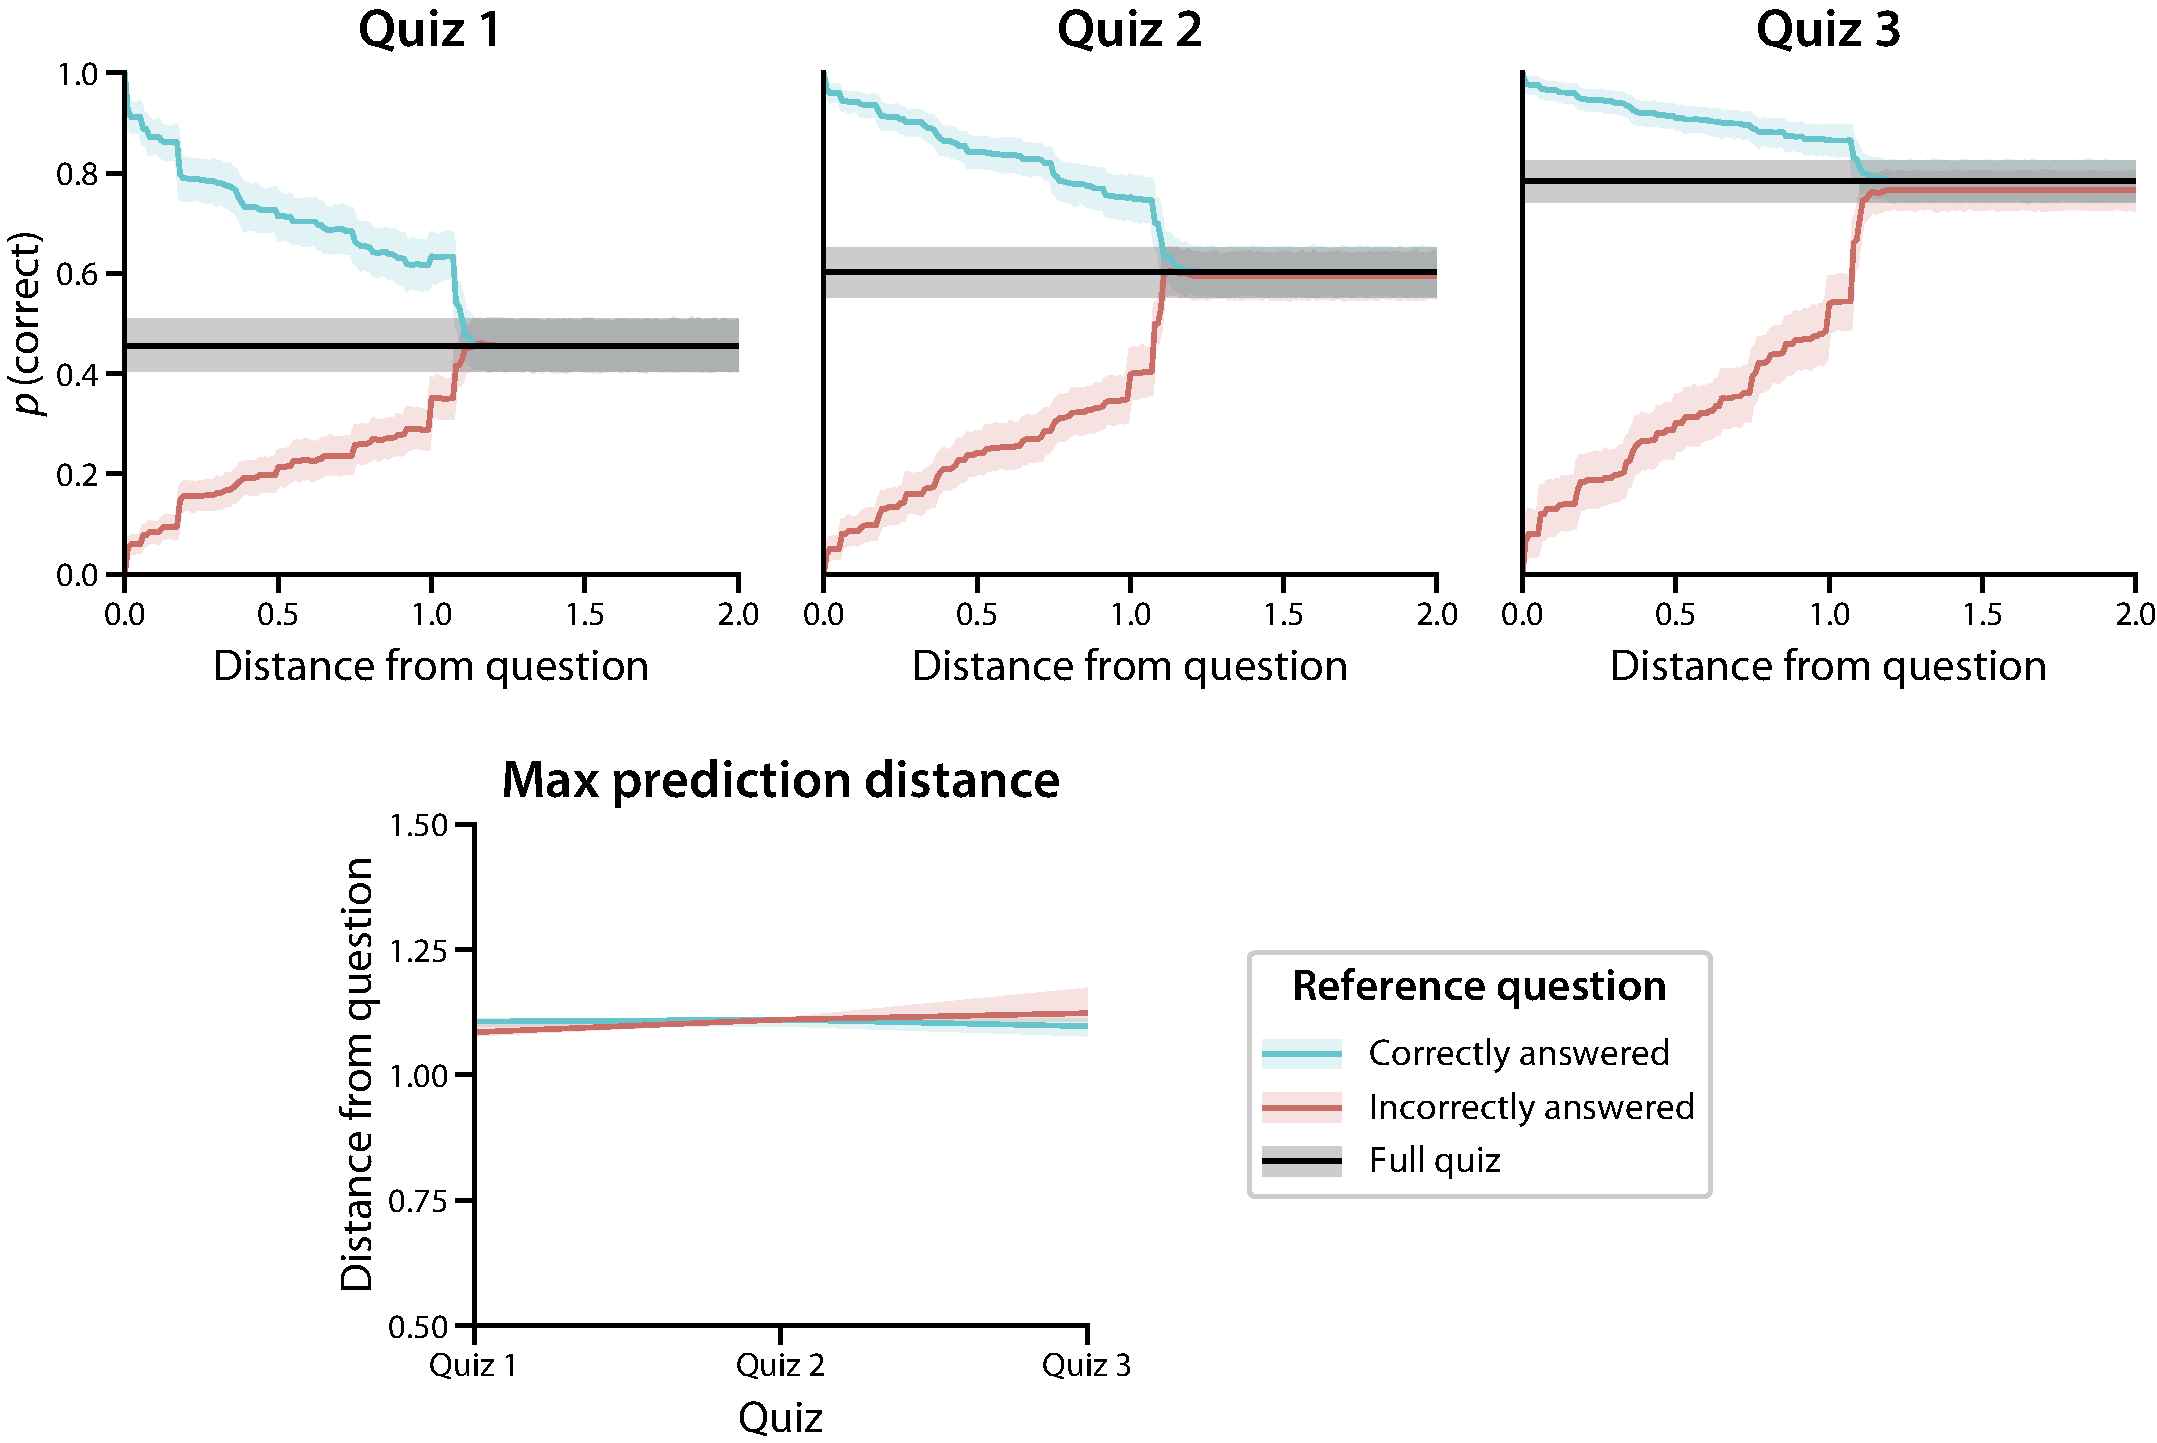
\includegraphics[width=0.8\textwidth]{figs/knowledge-smoothness}

    \caption{\textbf{Knowledge falls off gradually in text embedding space.}
    \textbf{A. Performance versus distance.} For each participant, for each
    correctly answered question (blue) or incorrectly answered question (red),
    we computed the proportion of correctly answered questions within a given
    distance of that question's embedding coordinate. We used these proportions
    as a proxy for participants' knowledge about the content within that region
    of the embedding space. We repeated this analysis for all questions and
    participants, and separately for each quiz (column). The black lines denote
    the average proportion correct across \textit{all} questions included in
    the analysis at the given distance. \textbf{B. Maximum distance for which
    performance is reliably different from the average.} We used a bootstrap
    procedure (see~\nameref{subsec:smoothness}) to estimate the point at which
    the blue and red lines in Panel A reliably diverged from the black line. We
    repeated this analysis separately for correctly and incorrectly answered
    questions from each quiz. \textbf{All panels.} Error ribbons denote
    bootstrap-estimated 95\% confidence intervals.}

    \label{fig:smoothness}
\end{figure}

With these ideas in mind, we asked: conditioned on answering a question
correctly, what proportion of all questions (within some radius, $r$, of that
question's embedding coordinate) were answered correctly? We plotted this
proportion as a function of $r$. Similarly, we could ask, conditioned on
answering a question incorrectly, how the proportion of correct responses
changed with $r$. As shown in Figure~\ref{fig:smoothness}, we found that quiz
performance falls off smoothly with distance, and the ``rate'' of the falloff
does not appear to change across the different quizzes, as measured by the
distance at which performance becomes statistically indistinguishable from a
simple proportion correct score (see~\nameref{subsec:smoothness}). This
suggests that, at least within the region of text embedding space covered by
the questions our participants answered (and as characterized using our topic
model), the rate at which knowledge changes with distance is relatively
constant, even as participants' overall level of knowledge varies across
quizzes or regions of the embedding space.

Knowledge estimates need not be limited to the content of the lectures. As
illustrated in Figure~\ref{fig:knowledge-maps}, our general approach to
estimating knowledge from a small number of quiz questions may be extended to
\textit{any} content, given its text embedding coordinate. To visualize how
knowledge ``spreads'' through text embedding space to content beyond the
lectures participants watched, we first fit a new topic model to the lectures'
sliding windows with $k = 100$~topics. Conceptually, increasing the
number of topics used by the model functions to increase the ``resolution'' of
the embedding space, providing a greater ability to estimate knowledge for
content that is highly similar to (but not precisely the same as) that
contained in the two lectures. We note that we used these 2D maps solely for
visualization; all relevant comparisons, distance computations, and statistical
tests we report above were carried out in the original 15-dimensional space,
using the 15-topic model. Aside from increasing the number of topics from 15 to
100, all other procedures and model parameters were carried over from the
preceding analyses. As in our other analyses, we resampled each lecture's topic
trajectory to 1~Hz and projected each question into a shared text embedding
space.

\begin{figure}[tp]
    \centering
    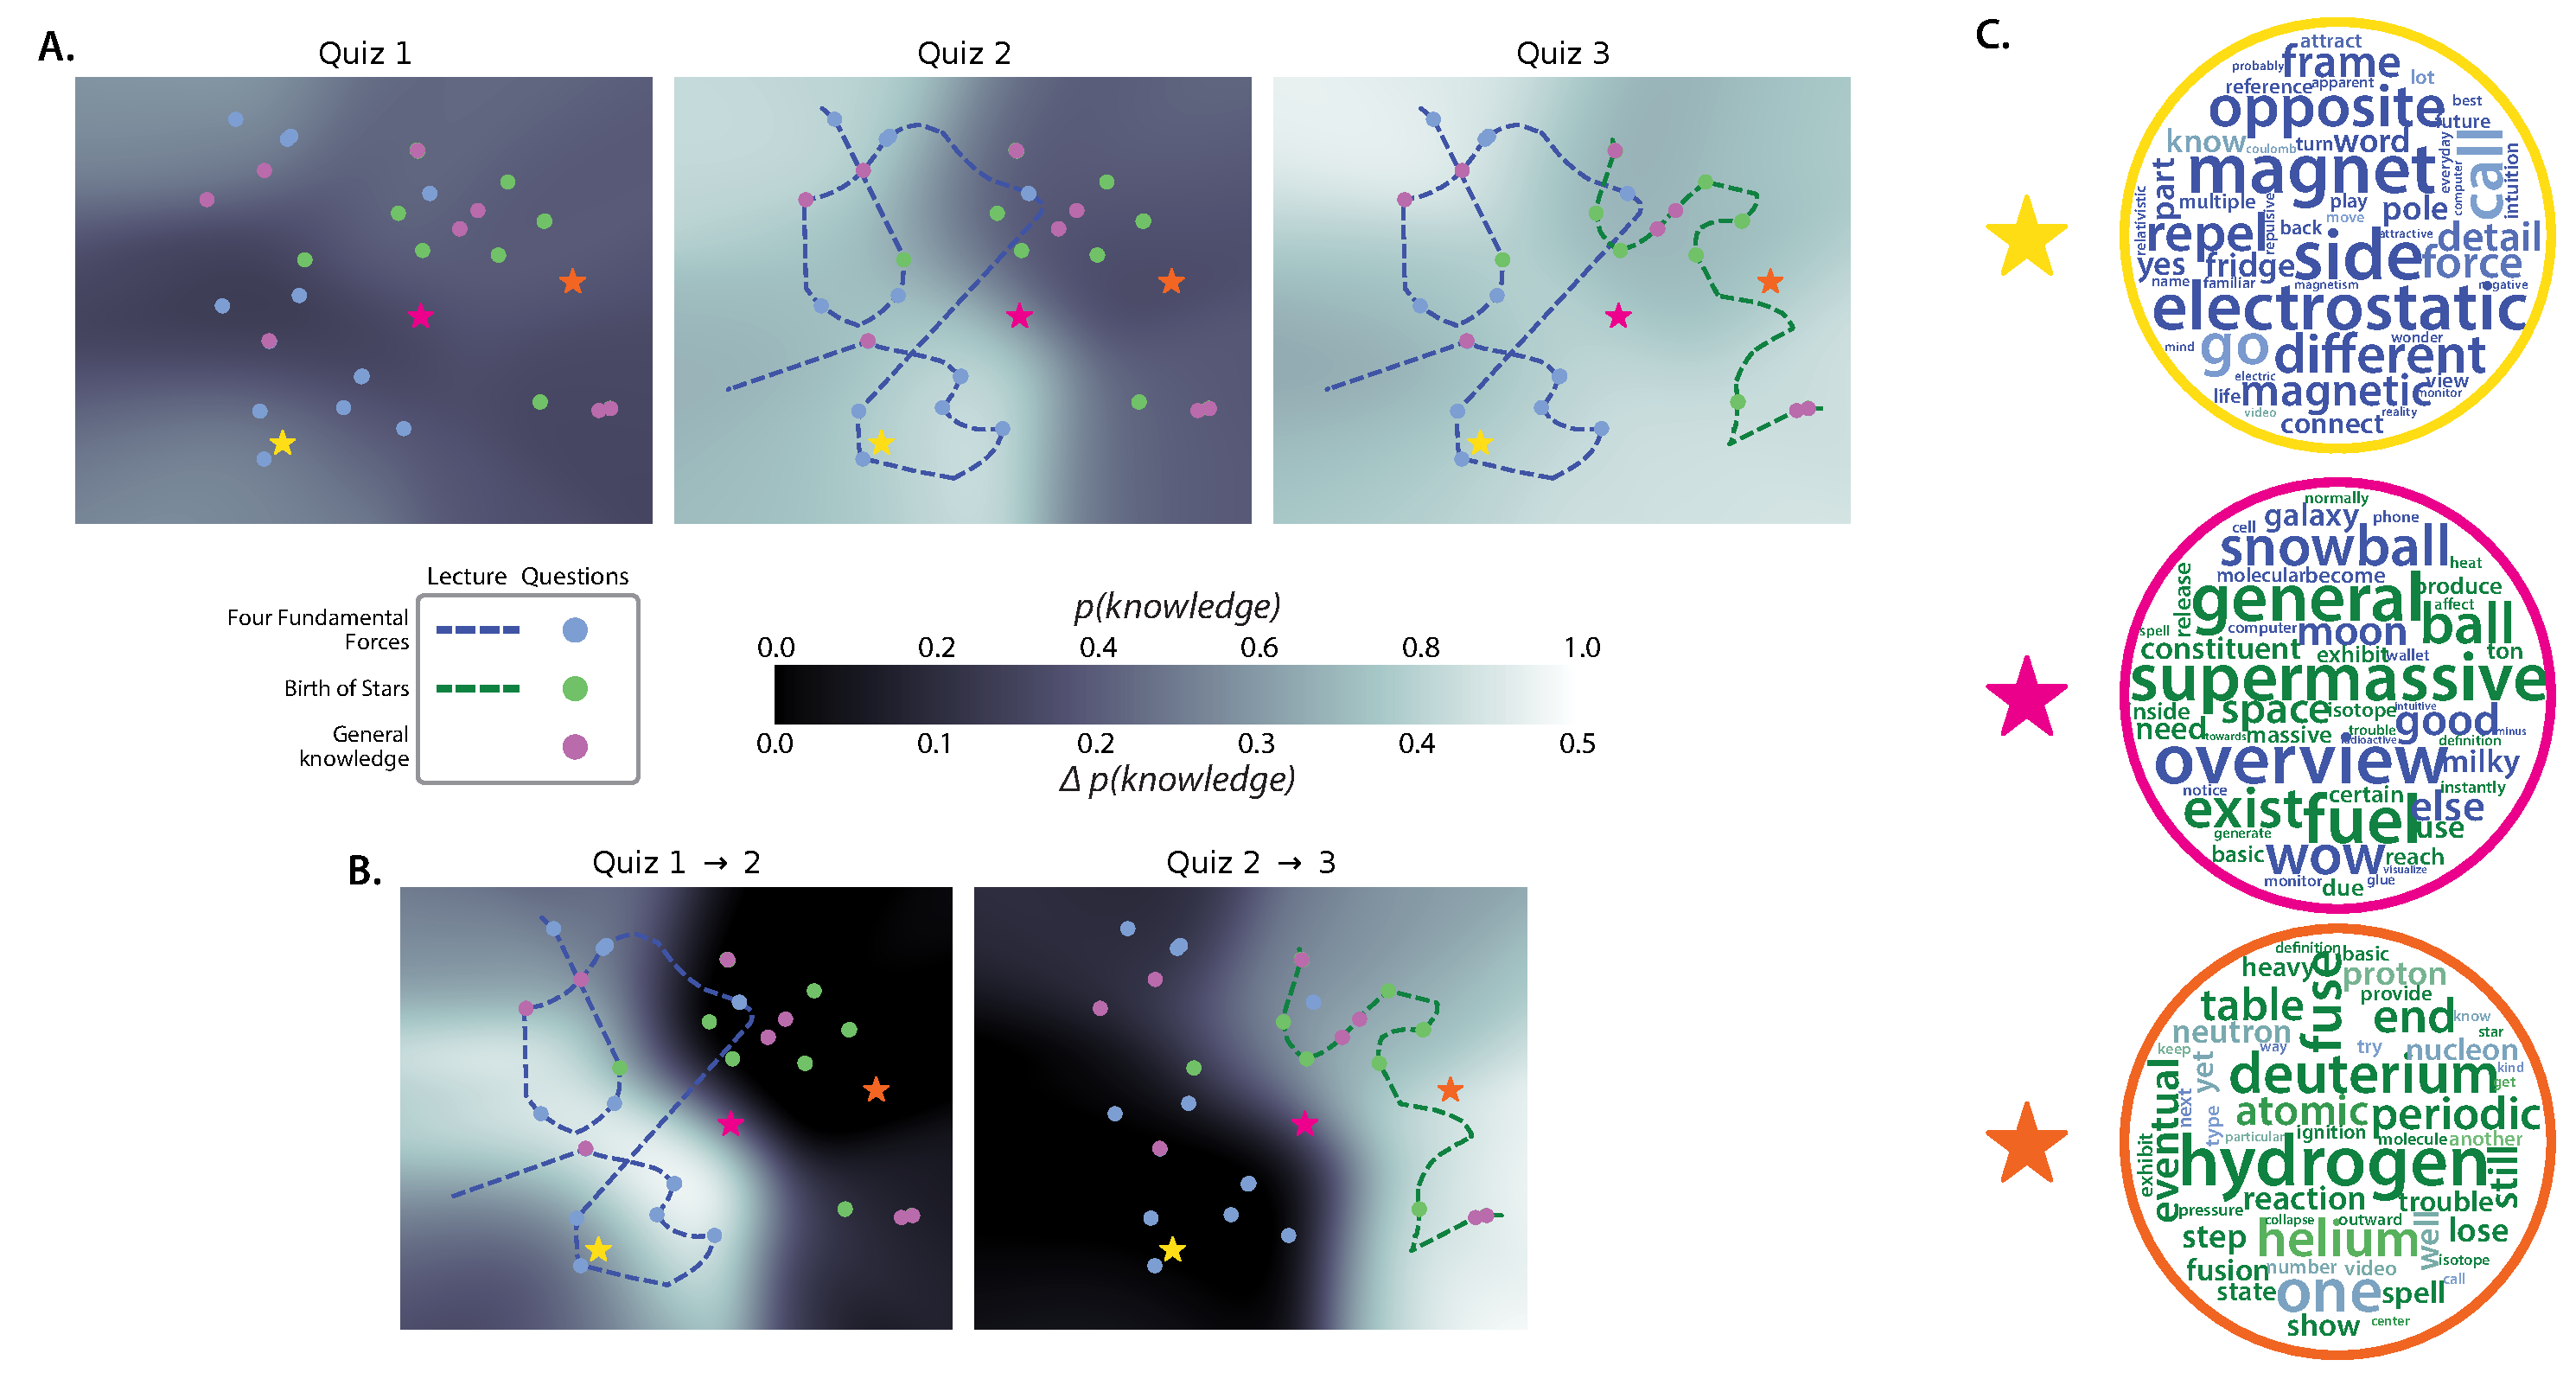
\includegraphics[width=\textwidth]{figs/knowledge_and_learning_maps}

    \caption{\textbf{Mapping out the geometry of knowledge and learning.}
    \textbf{A. Average ``knowledge maps'' estimated using each quiz.} Each map
    displays a 2D projection of the estimated knowledge about the content
    reflected by \textit{all} regions of topic space (see
    \nameref{subsec:knowledge-maps}). The topic trajectories of the two
    lectures are indicated by dotted lines (blue: Lecture 1; green: Lecture 2),
    and the coordinates of each question are indicated by dots (light blue:
    Lecture 1-related; light green: Lecture 2-related; purple: general physics
    knowledge). Each map reflects an average across all participants. For
    individual participants' maps, see Supplementary
    Figures~\individualKnowledgeMapsA,~\individualKnowledgeMapsB,
    and~\individualKnowledgeMapsC. \textbf{B. Average ``learning maps''
    estimated between each successive pair of quizzes.} The learning maps
    follow the same general format as the knowledge maps in Panel A, but here
    the shading at each coordinate indicates the \textit{difference} between
    the corresponding coordinates in the indicated \textit{pair} of knowledge
    maps---i.e., how much the estimated knowledge ``changed'' between the two
    quizzes. Each map reflects an average across all participants. For
    individual participants' maps, see Supplementary
    Figures~\individualLearningMapsA~and~\individualLearningMapsB. \textbf{C.
    Word clouds for sampled points in topic space.} Each word cloud displays
    the weighted blend of words underlying the topic proportions represented at
    the corresponding colored star's location on the maps. In each word cloud,
    the words' relative sizes correspond to their relative weights at the
    starred location, and their colors indicate their relative weights in
    \textit{Four Fundamental Forces} (blue) versus \textit{Birth of Stars}
    (green) lectures, on average, across all timepoints' topic vectors.}

    \label{fig:knowledge-maps}
    \end{figure}

We projected the resulting 100-dimensional topic vectors (for each second of
video and each quiz question) onto a shared 2-dimensional plane (see
\nameref{subsec:knowledge-maps}). Next, we sampled points from a $100 \times
100$ grid of coordinates that evenly tiled a rectangle enclosing the 2D
projections of the videos and questions. We used
Equation~\ref{eqn:rbf-knowledge} to estimate participants' knowledge at each of
these 10,000 sampled locations, and averaged these estimates across
participants to obtain an estimated average \textit{knowledge map}
(Fig.~\ref{fig:knowledge-maps}A). Intuitively, the knowledge map constructed
from a given quiz's responses provides a visualization of how ``much''
participants knew about any content expressible by the fitted text embedding
model at the point in time when they completed that quiz.

Several features of the resulting knowledge maps are worth noting. The average
knowledge map estimated from Quiz~1 responses (Fig.~\ref{fig:knowledge-maps}A,
leftmost map) shows that participants tended to have relatively little
knowledge about any parts of the text embedding space (i.e., the shading is
relatively dark everywhere). The knowledge map estimated from Quiz~2 responses
shows a marked increase in knowledge on the left side of the map (around
roughly the same range of coordinates traversed by the \textit{Four Fundamental
Forces} lecture, indicated by the dotted blue line). In other words,
participants' estimated increase in knowledge is localized to conceptual
content that is nearby (i.e., related to) the content from the lecture they
watched prior to taking Quiz~2. This localization is non-trivial: these
knowledge estimates are informed only by the embedded coordinates of the
\textit{quiz questions}, not by the embeddings of either lecture (see
Eqn.~\ref{eqn:rbf-knowledge}). Finally, the knowledge map estimated from Quiz~3
responses shows a second increase in knowledge, localized to the region
surrounding the embedding of the \textit{Birth of Stars} lecture participants
watched immediately prior to taking Quiz~3.

Another way of visualizing these content-specific increases in knowledge after
participants viewed each lecture is displayed in
Figure~\ref{fig:knowledge-maps}B. Taking the point-by-point difference between
the knowledge maps estimated from responses to a successive pair of quizzes
yields a \textit{learning map} that describes the \textit{change} in knowledge
estimates from one quiz to the next. These learning maps highlight that the
estimated knowledge increases we observed across maps were specific to the
regions around the embeddings of each lecture, in turn.

Because the 2D projection we used to construct the knowledge and learning maps
is invertible, we may gain additional insights into these maps' meanings by
reconstructing the original high-dimensional topic vector for any location on
the map we are interested in. For example, this could serve as a useful tool
for an instructor looking to better understand which content areas a student
(or a group of students) knows well (or poorly). As a demonstration, we show
the top-weighted words from the blends of topics reconstructed from three
example locations on the maps (Fig.~\ref{fig:knowledge-maps}C): one point near
the \textit{Four Fundamental Forces} embedding (yellow), a second point near
the \textit{Birth of Stars} embedding (orange), and a third point between the
two lectures' embeddings (pink). As shown in the word clouds in the panel, the
top-weighted words at the example coordinate near the \textit{Four Fundamental
Forces} embedding tended to be weighted more heavily by the topics expressed in
that lecture. Similarly, the top-weighted words at the example coordinate near
the \textit{Birth of Stars} embedding tended to be weighted more heavily by the
topics expressed in \textit{that} lecture. And the top-weighted words at the
example coordinate between the two lectures' embeddings show a roughly even mix
of words most strongly associated with each lecture.

\section*{Discussion}

We developed a computational framework that uses short multiple-choice quizzes
to gain nuanced insights into what learners know and how their knowledge
changes with training. First, we show that our approach can automatically match
the conceptual knowledge probed by individual quiz questions to the
corresponding moments in lecture videos when those concepts were presented
(Fig.~\ref{fig:question-correlations}). Next, we demonstrate how we can
estimate moment-by-moment ``knowledge traces'' that reflect the degree of
knowledge participants have about each video's time-varying content, and
capture temporally specific increases in knowledge after viewing each lecture
(Fig.~\ref{fig:knowledge-timeseries}). We also show that these knowledge
estimates can generalize to held-out questions (Fig.~\ref{fig:predictions}).
Finally, we use our framework to construct visual maps that provide snapshot
estimates of how much participants know about any concept within the scope of
our text embedding model, and how much their knowledge of those concepts
changes with training (Fig.~\ref{fig:knowledge-maps}).

We view our work as making several contributions to the study of how people
acquire conceptual knowledge. First, from a methodological standpoint, our
modeling framework provides a systematic means of mapping out and
characterizing knowledge in maps that have infinite (arbitrarily many) numbers
of coordinates, and of ``filling out'' those maps using relatively small
numbers of multiple choice quiz questions. Our experimental finding that we can
use these maps to predict responses to held-out questions has several
psychological implications as well. For example, concepts that are assigned to
nearby coordinates by the text embedding model also appear to be ``known to a
similar extent'' (as reflected by participants' responses to held-out
questions; Fig.~\ref{fig:predictions}). This suggests that participants also
\textit{conceptualize} similarly the content reflected by nearby embedding
coordinates. How participants' knowledge falls off with spatial distance is
captured by the knowledge maps we infer from their quiz responses
(e.g., Figs.~\ref{fig:smoothness},~\ref{fig:knowledge-maps}). In other words,
our study shows that knowledge about a given concept implies knowledge about
related concepts, and we also show how estimated knowledge falls off with
distance in text embedding space.

In our study, we characterize the ``coordinates'' of participants' knowledge
using a relatively simple ``bag of words'' text embedding model~\citep[LDA;
][]{BleiEtal03}. More sophisticated text embedding models, such as
transformer-based models~\citep{ViswEtal17, DevlEtal18, ChatGPT, TouvEtal23}
can learn complex grammatical and semantic relationships between words,
higher-order syntactic structures, stylistic features, and more. We considered
using transformer-based models in our study, but we found that the text
embeddings derived from these models were surprisingly uninformative with
respect to differentiating or otherwise characterizing the conceptual content
of the lectures and questions we used. We suspect that this reflects a broader
challenge in constructing models that are high-resolution within a given domain
(e.g., the domain of physics lectures and questions) \textit{and} sufficiently
broad so as to enable them to cover a wide range of domains. For example, we
found that the embeddings derived even from much larger and more modern models
like BERT~\citep{DevlEtal18}, GPT~\citep{ViswEtal17}, LLaMa~\citep{TouvEtal23},
and others that are trained on enormous text corpora, end up yielding poor
resolution within the content space spanned by individual course videos
(Supp.~Fig.~\ldaVsBERT). Whereas the LDA embeddings of the lectures and
questions are ``near'' each other (i.e., the convex hull enclosing the two
lectures' trajectories is highly overlapping with the convex hull enclosing the
questions' embeddings), the BERT embeddings of the lectures and questions are
instead largely distinct (top row of Supp.~Fig.~\ldaVsBERT). The LDA embeddings
of the questions for each lecture and the corresponding lecture's trajectory
are also similar. For example, as shown in Fig.~\ref{fig:sliding-windows}C, the
LDA embeddings for \textit{Four Fundamental Forces} questions (blue dots)
appear closer to the \textit{Four Fundamental Forces} lecture trajectory (blue
line), whereas the LDA embeddings for \textit{Birth of Stars} questions (green
dots) appear closer to the \textit{Birth of Stars} lecture trajectory (green
line). The BERT embeddings of the lectures and questions do not show this
property (Supp.~Fig.~\ldaVsBERT). We also examined per-question ``content
matches'' between individual questions and individual moments of each lecture
(Figs.~\ref{fig:question-correlations},~\ldaVsBERT). The time series plot of
individual questions' correlations are different from each other when computed
using LDA (e.g., the traces can be clearly visually separated), whereas the
correlations computed from BERT embeddings of different questions all look very
similar. This tells us that LDA is capturing some differences in content
between the questions, whereas BERT is not. The time series plots of individual
questions' correlations have clear ``peaks'' when computed using LDA, but not
when computed using BERT. This tells us that LDA is capturing a ``match''
between the content of each question and a relatively well-defined time window
of the corresponding lectures. The BERT embeddings appear to blur together the
content of the questions versus specific moments of each lecture. Finally, we
also compared the pairwise correlations between embeddings of questions within
versus across content areas (i.e., content covered by the individual lectures,
lecture-specific questions, and by the ``general physics knowledge''
questions). The LDA embeddings show a strong contrast between same-content
embeddings versus across-content embeddings. In other words, the embeddings of
questions about the \textit{Four Fundamental Forces} material are highly
correlated with the embeddings of the \textit{Four Fundamental Forces} lecture,
but not with the embeddings of \textit{Birth of Stars}, questions about
\textit{Birth of Stars}, or general physics knowledge questions. We see a
similar pattern with the LDA embeddings of the \textit{Birth of Stars}
questions (Fig.~\ref{fig:topics}, Supp.~Fig.~\topicWeights). In contrast, the
BERT embeddings are all highly correlated with each other (Supp.
Fig.~\ldaVsBERT). Taken together, these comparisons illustrate how LDA (trained
on the specific content in question) provides both coverage of the requisite
material and specificity at the level of the content covered by individual
questions. BERT, on the other hand, essentially assigns both lectures and all
of the questions (which are all broadly about ``physics'') into a tiny region
of its embedding space, thereby blurring out meaningful distinctions between
different specific concepts covered by the lectures and questions. We note that
these are not criticisms of BERT (or other large language models trained on
large and diverse corpora). Rather, our point is that simple fine-tuned models
trained on a relatively small but specialized corpus can outperform much more
complicated models trained on much larger corpora, when we are specifically
interested in capturing subtle conceptual differences at the level of a single
course lecture or question. Of course if our goal had been to find a model that
generalized to many different content areas, we would expect our approach to
perform comparatively poorly relative to BERT or other much larger models. We
suggest that bridging the tradeoff between high resolution within each content
area versus the ability to generalize to many different content areas will be
an important challenge for future work in this domain.

Another application for large language models that does \textit{not} require
explicitly modeling the content of individual lectures or questions is to
leverage the models' abilities to generate text. For example, generative text
models like ChatGPT~\citep{ChatGPT} and LLaMa~\citep{TouvEtal23} are already
being used to build a new generation of interactive tutoring
systems~\citep[e.g.,][]{MannEtal23b}. Unlike the approach we have taken here,
these generative text model-based systems do not explicitly model what learners
know, or how their knowledge changes over time with training. One could imagine
building a hybrid system that combines the best of both worlds: a large
language model that can \textit{generate} text, combined with a smaller model
that can \textit{infer} what learners know and how their knowledge changes over
time. Such a hybrid system could potentially be used to build the next
generation of interactive tutoring systems that are able to adapt to learners'
needs in real time, and that are able to provide more nuanced feedback about
what learners know and what they do not know.

At the opposite end of the spectrum from large language models, one could also
imagine \textit{simplifying} some aspects of our LDA-based approach by
computing simple word overlap metrics. For example, the Jaccard similarity
between text $A$ and $B$ is computed as the number of unique words in the
intersection of words from $A$ and $B$ divided by the number of unique words in
the union of words from $A$ and $B$. In a supplementary analysis (Supp.
Fig.~\jaccard), we compared the LDA-based question-lecture matches we reported
in Figure~\ref{fig:question-correlations} with the Jaccard similarities between
each question and each sliding window of text from the corresponding lecture.
As shown in Supplementary Figure~\jaccard, this simple word-matching approach
does not appear to capture the same level of specificity as the LDA-based
approach. Whereas the LDA-based approach often yields a clear peak in the
time series of correlations between each question and the corresponding lecture,
the Jaccard similarity-based approach does not. Furthermore, these LDA-based
matches appear to capture conceptual overlaps between the questions and
lectures (Supp.~Tab.~\matchTab), whereas simple word matching does not. For
example, one of the example questions examined in Supplementary
Figure~\jaccard~asks ``Which of the following occurs as a cloud of atoms gets
more dense?'' The LDA-based matches identify lecture timepoints where the
relevant \textit{topics} are discussed (e.g., when words like ``cloud,''
``atom,'' ``dense,'' etc., are mentioned \textit{together}). The Jaccard
similarity-based matches, on the other hand, are strong when \textit{any} of
these words are mentioned, even if they do not occur together.

We view our approach as occupying a sort of ``sweet spot,'' between much larger
language models and simple word matching-based approaches, that enables us to
capture the relevant conceptual content of course materials at an appropriate
semantic scale. Our approach enables us to accurately and consistently identify
each question's content in a way that also matches up with what is presented in
the lectures. In turn, this enables us to construct accurate predictions about
participants' knowledge of the conceptual content tested by held-out questions
(Fig.~\ref{fig:predictions}).

One limitation of our approach is that topic models contain no explicit
internal representations of more complex aspects of ``knowledge,'' like
knowledge graphs, dependencies or associations between concepts, causality, and
so on. These representations might (in principle) be added as extensions to our
approach to more accurately and precisely capture, characterize, and track
learners' knowledge. However, modeling these aspects of knowledge will likely
require substantial additional research effort.

Within the past several years, the global pandemic forced many educators to
suddenly adapt to teaching remotely~\citep{MoseEtal21, ShimLee20, KawaEtal21,
Whal20}. This change in world circumstances is happening alongside (and perhaps
accelerating) geometric growth in the availability of high-quality online
courses from platforms such as Khan Academy~\citep{Khan04},
Coursera~\citep{Youn12}, EdX~\citep{Kolo13}, and others~\citep{RhoaEtal13}.
Continued expansion of the global internet backbone and improvements in
computing hardware have also facilitated improvements in video streaming,
enabling videos to be easily shared and viewed by increasingly large segments
of the world's population. This exciting time for online course instruction
provides an opportunity to re-evaluate how we, as a global community, educate
ourselves and each other. For example, we can ask: what defines an effective
course or training program? Which aspects of teaching might be optimized and/or
augmented by automated tools? How and why do learning needs and goals vary
across people? How might we lower barriers to receiving a high-quality
education?

Alongside these questions, there is a growing desire to extend existing
theories beyond the domain of lab testing rooms and into real
classrooms~\citep{Kauf03}. In part, this has led to a recent resurgence of
``naturalistic'' or ``observational'' experimental paradigms that attempt to
better reflect more ethologically valid phenomena that are more directly
relevant to real-world situations and behaviors~\citep{NastEtal20}. In turn,
this has brought new challenges in data analysis and interpretation. A key step
towards solving these challenges will be to build explicit models of real-world
scenarios and how people behave in them (e.g., models of how people learn
conceptual content from real-world courses, as in our current study). A second
key step will be to understand which sorts of signals derived from behaviors
and/or other measurements~\citep[e.g., neurophysiological data; ][]{NguyEtal22,
MeshEtal20, PoulEtal17, BeviEtal19, DikkEtal17} might help to inform these
models. A third major step will be to develop and employ reliable ways of
evaluating the complex models and data that are a hallmark of naturalistic
paradigms.

Beyond specifically predicting what people \textit{know}, the fundamental ideas
we develop here also relate to the notion of ``theory of mind'' of other
individuals~\citep{GoldWinn12, KansEtal15, Melt11}. Considering others' unique
perspectives, prior experiences, knowledge, goals, etc., can help us to more
effectively interact and communicate~\citep{ShaoEtal18, StepBaer06, Ratk18}.
One could imagine future extensions of our work (e.g., analogous to the
knowledge and learning maps shown in Fig.~\ref{fig:knowledge-maps}), that
attempt to characterize how well-aligned different people's knowledge bases or
backgrounds are. In turn, this might be used to model how knowledge (or other
forms of communicable information) flows not just between teachers and
students, but between friends having a conversation, individuals on a first
date, participants at a business meeting, doctors and patients, experts and
non-experts, political allies or adversaries, and more. For example, the extent
to which two people's knowledge maps ``match'' or ``align'' in a given region
of text embedding space might serve as a predictor of how effectively they will
be able to communicate about the corresponding conceptual content.

Ultimately, our work suggests a rich new line of questions about the geometric
``form'' of knowledge, how knowledge changes over time, and how we might map
out the full space of what an individual knows. Our finding that detailed
estimates about knowledge may be obtained from short quizzes shows one way that
traditional approaches to evaluation in education may be extended. We hope that
these advances might help pave the way for new approaches to teaching or
delivering educational content that are tailored to individual students'
learning needs and goals.

\section*{Materials and methods}

\subsection*{Participants}

We enrolled a total of 50 Dartmouth undergraduate students in our study.
Participants received optional course credit for enrolling. We asked each
participant to complete a demographic survey that included questions about
their age, gender, native spoken language, ethnicity, race, hearing, color
vision, sleep, coffee consumption, level of alertness, and several aspects of
their educational background and prior coursework.

Participants' ages ranged from 18 to 22 years (mean: 19.52 years; standard
deviation: 1.09 years). A total of 15 participants reported their gender as
male and 35 participants reported their gender as female. A total of 49
participants reported their native language as ``English'' and 1 reported
having another native language. A total of 47 participants reported their
ethnicity as ``Not Hispanic or Latino'' and three reported their ethnicity as
``Hispanic or Latino.'' Participants reported their races as White (32
participants), Asian (14 participants), Black or African American (5
participants), American Indian or Alaska Native (1 participant), and Native
Hawaiian or Other Pacific Islander (1 participant). (Note that some
participants selected multiple racial categories.)

A total of 49 participants reporting having normal hearing and 1 participant
reported having some hearing impairment. A total of 49 participants reported
having normal color vision and 1 participant reported being color blind.
Participants reported having had, on the night prior to testing, 2--4 hours of
sleep (1 participant), 4--6 hours of sleep (9 participants), 6--8 hours of
sleep (35 participants), or $8+$ hours of sleep (5 participants). They reported
having consumed, on the same day and leading up to their testing session, 0
cups of coffee (38 participants), 1 cup of coffee (10 participants), 3 cups of
coffee (1 participant), or $4+$ cups of coffee (1 participant).

No participants reported that their focus was currently impaired (e.g., by
drugs or alcohol). Participants reported their current level of alertness, and
we converted their responses to numerical scores as follows: ``very sluggish''
(-2), ``a little sluggish'' (-1), ``neutral'' (0), ``fairly alert'' (1), and
``very alert'' (2). Across all participants, a range of alertness levels were
reported (range: -2--1; mean: -0.10; standard deviation: 0.84).

Participants reported their undergraduate major(s) as ``social sciences'' (28
participants), ``natural sciences'' (16 participants), ``professional'' (e.g.,
pre-med or pre-law; 8 participants), ``mathematics and engineering'' (7
participants), ``humanities'' (4 participants), or ``undecided'' (3
participants). Note that some participants selected multiple categories for
their undergraduate major(s). We also asked participants about the courses they
had taken. In total, 45 participants reported having taken at least one Khan
Academy course in the past, and 5 reported not having taken any Khan Academy
courses. Of those who reported having watched at least one Khan Academy course,
7 participants reported having watched 1--2 courses, 11 reported having watched
3--5 courses, 8 reported having watched 5--10 courses, and 19 reported having
watched 10 or more courses. We also asked participants about the specific
courses they had watched, categorized under different subject areas. In the
``Mathematics'' area, participants reported having watched videos on AP
Calculus AB (21 participants), Precalculus (17 participants), Algebra 2 (14
participants), AP Calculus BC (12 participants), Trigonometry (11
participants), Algebra 1 (10 participants), Geometry (8 participants),
Pre-algebra (7 participants), Multivariable Calculus (5 participants),
Differential Equations (5 participants), Statistics and Probability (4
participants), AP Statistics (2 participants), Linear Algebra (2 participants),
Early Math (1 participant), Arithmetic (1 participant), and other videos not
listed in our survey (5 participants). In the ``Science and engineering'' area,
participants reported having watched videos on Chemistry, AP Chemistry, or
Organic Chemistry (21 participants); Physics, AP Physics I, or AP Physics II
(18 participants); Biology, AP Biology; or High school Biology (15
participants); Health and Medicine (1 participant); or other videos not listed
in our survey (5 participants). We also asked participants whether they had
specifically seen the videos used in our experiment. Of the 45 participants who
reported having having taken at least one Khan Academy course in the past, 44
participants reported that they had not watched the \textit{Four Fundamental
Forces} video, and 1 participant reported that they were not sure whether they
had watched it. All participants reported that they had not watched the
\textit{Birth of Stars} video. When we asked participants about non-Khan
Academy online courses, they reported having watched or taken courses on
Mathematics (15 participants), Science and engineering (11 participants), Test
preparation (9 participants), Economics and finance (3 participants), Arts and
humanities (2 participants), Computing (2 participants), and other categories
not listed in our survey (17 participants). Finally, we asked participants
about in-person courses they had taken in different subject areas. They
reported taking courses in Mathematics (38 participants), Science and
engineering (37 participants), Arts and humanities (34 participants), Test
preparation (27 participants), Economics and finance (26 participants),
Computing (14 participants), College and careers (7 participants), or other
courses not listed in our survey (6 participants).


\subsection*{Experiment}\label{subsec:experiment}

We hand-selected two course videos from the Khan Academy platform: \textit{Four
Fundamental Forces} (an introduction to gravity, electromagnetism, the weak
nuclear force, and the strong nuclear force; duration: 10 minutes and 29
seconds) and \textit{Birth of Stars} (an introduction to how stars are formed;
duration: 7 minutes and 57 seconds). All participants viewed the videos in the
same order (i.e., \textit{Four Fundamental Forces} followed by \textit{Birth of
Stars}).

We then hand-created 39 multiple-choice questions: 15 about the conceptual
content of \textit{Four Fundamental Forces} (i.e., Lecture~1), 15 about the
conceptual content of \textit{Birth of Stars} (i.e., Lecture~2), and 9
questions that tested for general conceptual knowledge about basic physics
(covering material that was not presented in either video). To help broaden the
set of lecture-specific questions, our team worked through each lecture in
small segments to identify what each segment was ``about'' conceptually, and
then write a question about that concept. The general physics questions were
drawn our team's prior coursework and areas of interest, along with internet
searches and brainstorming with the project team and other members of J.R.M.'s
lab. Although we attempted to design the questions to test ``conceptual
knowledge,'' we note that estimating the specific ``amount'' of conceptual
understanding that each question ``requires'' to answer is somewhat subjective,
and might even come down to the ``strategy'' a given participant uses to answer
the question at that particular moment. The full set of questions and answer
choices may be found in Supplementary Table~\questions.  The final set of
questions (and response options) was reviewed and approved by J.R.M. before we
collected or analyzed the text or experimental data.

Over the course of the experiment, participants completed three 13-question
multiple-choice quizzes: the first before viewing Lecture~1, the second between
Lectures~1 and 2, and the third after viewing Lecture~2 (see
Fig.~\ref{fig:experiment}). The questions appearing on each quiz, for each
participant, were randomly chosen from the full set of 39, with the constraints
that (a) each quiz contained exactly 5 questions about Lecture~1, 5 questions
about Lecture~2, and 3 questions about general physics knowledge, and (b) each
question appear exactly once for each participant. The orders of questions on
each quiz, and the orders of answer options for each question, were also
randomized. We obtained informed consent from all participants, and our
experimental protocol was approved by the Committee for the Protection of Human
Subjects at Dartmouth College. We used this experiment to develop and test our
computational framework for estimating knowledge and learning.

\subsection*{Analysis}

\subsubsection*{Statistics}

All of the statistical tests performed in our study were two-sided. The 95\%
confidence intervals we reported for each correlation were estimated by
generating 10,000 bootstrap distributions of correlation coefficients by
sampling (with replacement) from the observed data.

\subsubsection*{Constructing text embeddings of multiple lectures and questions}\label{subsec:topic-modeling}

We adapted an approach we developed in prior work~\citep{HeusEtal21} to embed
each moment of the two lectures and each question in our pool in a common
representational space. Briefly, our approach uses a topic model~\citep[Latent
Dirichlet Allocation; ][]{BleiEtal03} trained on a set of documents, to
discover a set of $k$ ``topics'' or ``themes.'' Formally, each topic is
defined as a distribution of weights over words in the model's vocabulary
(i.e., the union of all unique words, across all documents, excluding ``stop
words.''). Conceptually, each topic is intended to give larger weights to words
that are semantically related (as inferred from their tendency to co-occur in
the same document). After fitting a topic model, each document in the training
set, or any \textit{new} document that contains at least some of the words in
the model's vocabulary, may be represented as a $k$-dimensional vector
describing how much the document (most probably) reflects each topic. To select
an appropriate $k$ for our model, as a starting point, we identified the
minimum number of topics that yielded at least one ``unused'' topic (i.e., in
which all words in the vocabulary were assigned uniform weights) after
training. This indicated that the number of topics was sufficient to capture
the set of latent themes present in the two lectures (from which we constructed
our document corpus, as described below). We found this value to be $k = 15$
topics. We found that with a limited number of additional adjustments
following~\citep{BoydEtal14}, such as removing corpus-specific stop-words, the
model yielded (subjectively) sensible and coherent topics. The distribution of
weights over words in the vocabulary for each discovered topic is shown in
Supplementary Figure~\topicWordWeights, and each topic's top-weighted words may
be found in Supplementary Table~\topics.

As illustrated in Figure~\ref{fig:sliding-windows}A, we start by building up a
corpus of documents using overlapping sliding windows that span each video's
transcript. Khan Academy provides professionally created, manual transcriptions
of all videos for closed captioning. However, such transcripts would not be
readily available in all contexts to which our framework could potentially be
applied. Khan Academy videos are hosted on the YouTube platform, which
additionally provides automated captions. We opted to use these automated
transcripts~\citep[which, in prior work, we have found to be of sufficiently
near-human quality to yield reliable data in behavioral
studies; ][]{ZimaEtal18} when developing our framework in order to make
it more directly extensible and adaptable by others in the future.

We fetched these automated transcripts using the
\texttt{youtube-transcript-api} Python package~\citep{Depo18}. The transcripts
consisted of one timestamped line of text for every few seconds (mean: 2.34~s;
standard deviation: 0.83~s) of spoken content in the video (i.e., corresponding
to each individual caption that would appear on-screen if viewing the lecture
via YouTube, and when those lines would appear). We defined a sliding window
length of (up to) $w = 30$ transcript lines, and assigned each window a
timestamp corresponding to the midpoint between the timestamps for its first
and last lines. This $w$ parameter was chosen to match the same number of words
per sliding window (rounded to the nearest whole word, and before
preprocessing) as the sliding windows we defined in our prior
work~\citep{HeusEtal21} (i.e., 185 words per sliding window).

These sliding windows ramped up and down in length at the beginning and end of
each transcript, respectively. In other words, each transcript's first sliding
window covered only its first line, the second sliding window covered the first
two lines, and so on. This ensured that each line from the transcripts appeared
in the same number ($w$) of sliding windows. We next performed a series of
standard text preprocessing steps: normalizing case, lemmatizing, removing
punctuation and removing stop-words. We constructed our corpus of stop words by
augmenting the Natural Language Toolkit~\citep[NLTK; ][]{BirdEtal09} English
stop word list with the following additional words, selected using one of the
approaches suggested by~\citep{BoydEtal14}: ``actual,'' ``actually,'' ``also,''
``bit,'' ``could,'' ``e,'' ``even,'' ``first,'' ``follow,'' ``following,''
``four,'' ``let,'' ``like,'' ``mc,'' ``really,'', ``saw,'' ``see,'' ``seen,''
``thing,'' and ``two.'' This yielded sliding windows with an average of 73.8
remaining words, and lasting for an average of 62.22~seconds. We treated the
text from each sliding window as a single ``document,'' and combined these
documents across the two videos' windows to create a single training corpus for
the topic model.

After fitting a topic model to the two videos' transcripts, we could use the
trained model to transform arbitrary (potentially new) documents into
$k$-dimensional topic vectors. A convenient property of these topic vectors is
that documents that reflect similar blends of topics (i.e., documents that
reflect similar themes, according to the model) will yield similar coordinates
(in terms of correlation, cosine similarity, Kullback-Leibler divergence,
Euclidean distance, or other geometric measures). In general, the similarity
between different documents' topic vectors may be used to characterize the
similarity in conceptual content between the documents.

We transformed each sliding window's text into a topic vector, and then used
linear interpolation (independently for each topic dimension) to resample the
resulting time series to one vector per second. We also used the fitted model to
obtain topic vectors for each question in our pool (see Supp.~Tab.~\questions).
Taken together, we obtained a \textit{trajectory} for each video, describing
its path through topic space, and a single coordinate for each question
(Fig.~\ref{fig:sliding-windows}C). Embedding both videos and all of the
questions using a common model enables us to compare the content from different
moments of videos, compare the content across videos, and estimate potential
associations between specific questions and specific moments of video.


\subsubsection*{Estimating dynamic knowledge traces}\label{subsec:traces}

We used the following equation to estimate each participant's knowledge about
timepoint $t$ of a given lecture, $\hat{k}(t)$:
\begin{equation}
    \hat{k}\left(f(t, L)\right) = \frac{\sum_{i \in \mathrm{correct}}\mathrm{ncorr}\left(f(t, L), f(i, Q)\right)}{\sum_{j = 1}^N \mathrm{ncorr}\left(f(t, L), f(j, Q)\right)},
    \label{eqn:prop}
\end{equation}
where

\begin{equation}
    \mathrm{ncorr}(x, y) = \frac{\mathrm{corr}(x, y) - \mathrm{mincorr}}{\mathrm{maxcorr} - \mathrm{mincorr}},
\end{equation}
and where $\mathrm{mincorr}$ and $\mathrm{maxcorr}$ are the minimum and maximum
correlations between any lecture timepoint and question, taken over all
timepoints in the given lecture, and all five questions \textit{about} that lecture appearing on the given quiz.
We also define $f(s, \Omega)$ as the
$s$\textsuperscript{th} topic vector from the set of topic vectors $\Omega$.
Here $t$ indexes the set of lecture topic vectors, $L$, and $i$ and $j$ index
the topic vectors of questions used to estimate the knowledge trace, $Q$. Note
that ``correct'' denotes the set of indices of the questions the participant
answered correctly on the given quiz.

Intuitively, $\mathrm{ncorr}(x, y)$ is the correlation between two topic
vectors (e.g., the topic vector from one timepoint in a lecture, $x$, and the
topic vector for one question, $y$), normalized by the minimum and maximum
correlations (across all timepoints $t$ and questions $Q$) to range between 0
and 1, inclusive. Equation~\ref{eqn:prop} then computes the weighted average
proportion of correctly answered questions about the content presented at
timepoint $t$, where the weights are given by the normalized correlations
between timepoint $t$'s topic vector and the topic vectors for each question.
The normalization step (i.e., using $\mathrm{ncorr}$ instead of the raw
correlations) ensures that every question contributes some non-negative amount
to the knowledge estimate.

\subsubsection*{GLMM METHODS SECTION PLACEHOLDER}\label{subsec:glmm}

\subsubsection*{Estimating the ``smoothness'' of knowledge}\label{subsec:smoothness}

In the analysis reported in Figure~\ref{fig:smoothness}A, we show how
participants' ability to correctly answer quiz questions changes as a function
of distance from a given correctly or incorrectly answered reference question.
We used a bootstrap-based approach to estimate the maximum distances over which
these proportions of correctly answered questions could be reliably
distinguished from participants' overall average proportion of correctly
answered questions.

For each of 10,000 iterations, we drew a random subsample (with replacement) of
50 participants from our dataset. Within each iteration, we first computed the
95\% confidence interval (CI) of the across-subsample-participants mean
proportion correct on each of the three quizzes, separately. To compute this
interval for each quiz, we repeatedly (1,000 times) subsampled participants
(with replacement, from the outer subsample for the current iteration) and
computed the mean proportion correct of each of these inner subsamples. We then
identified the 2.5\textsuperscript{th} and 97.5\textsuperscript{th} percentiles
of the resulting distributions of 1,000 means. These three intervals (one for
each quiz) served as our thresholds for confidence that the proportion correct
within a given distance from a reference question was reliably different (at
the $p < 0.05$ significance level) from the average proportion correct across
all questions on the given quiz.

Next, for each participant in the current subsample, and for each of the three
quizzes they completed (separately), we iteratively treated each of the 15
questions appearing on the given quiz as the ``reference'' question. We
constructed a series of concentric 15-dimensional ``spheres'' centered on the
reference question's embedding space coordinate, where each successive sphere's
radius increased by 0.01 (correlation distance) between 0 and 2, inclusive
(i.e., tiling the range of possible correlation distances with 201 spheres in
total). We then computed the proportion of questions enclosed within each
sphere that the participant answered correctly, and averaged these per-radius
proportion correct scores across reference questions that were answered
correctly, and those that were answered incorrectly. This resulted in two
number-of-spheres sequences of proportion-correct scores for each subsample
participant and quiz: one derived from correctly answered reference questions,
and one derived from incorrectly answered reference questions.

We computed the across-subsample-participants mean proportion correct for each
radius value (i.e., sphere) and ``correctness'' of reference question. This
yielded two sequences of proportion-correct scores for each quiz, analogous to
the blue and red lines displayed in Figure~\ref{fig:smoothness}A, but for the
present subsample. For each quiz, we then found the minimum distance from the
reference question (i.e., sphere radius) at which each of these two sequences
of per-radius proportion correct scores intersected the 95\% confidence
interval for the overall proportion correct (i.e., analogous to the black error
bands in Fig.~\ref{fig:smoothness}A).

This resulted in two ``intersection'' distances for each quiz (for correctly
answered and incorrectly answered reference questions). Repeating this full
process for each of the 10,000 bootstrap iterations output two distributions of
intersection distances for each of the three quizzes. The means and 95\%
confidence intervals for these distributions are plotted in
Figure~\ref{fig:smoothness}B.

\subsubsection*{Creating knowledge and learning map visualizations}\label{subsec:knowledge-maps}

An important feature of our approach is that, given a trained text embedding
model and participants' quiz performance on each question, we can estimate
their knowledge about \textit{any} content expressible by the embedding
model---not solely the content explicitly probed by the quiz questions, or even
appearing in the lectures. To visualize these estimates
(Fig.~\ref{fig:knowledge-maps}, Supp.
Figs.~\individualKnowledgeMapsA,~\individualKnowledgeMapsB,~\individualKnowledgeMapsC,~\individualLearningMapsA,
and~\individualLearningMapsB), we used Uniform Manifold Approximation and
Projection~\citep[UMAP; ][]{McInEtal18a, McInEtal18b} to construct a 2D
projection of the text embedding space. Whereas our main analyses used a
15-topic embedding space, we used a 100-topic embedding space for these
visualizations. This change in the number of topics overcame an undesirable
behavior in the UMAP embedding procedure, whereby embedding coordinates for the
15-topic model tended to be ``clumped'' into separated clusters, rather than
forming a smooth trajectory through the 2D space. When we increased the number
of topics to 100, the embedding coordinates in the 2D space formed a smooth
trajectory through the space, with substantially less clumping
(Fig.~\ref{fig:knowledge-maps}). Creating a ``map'' by sampling this
100-dimensional space at high resolution to obtain an adequate set of topic
vectors spanning the embedding space would be computationally intractable.
However, sampling a 2D grid is trivial.

At a high level, the UMAP algorithm obtains low-dimensional embeddings by
minimizing the cross-entropy between the pairwise (clustered) distances between
the observations in their original (e.g., 100-dimensional) space and the
pairwise (clustered) distances in the low-dimensional embedding space (in our
approach, the embedding space is 2D). In our implementation, pairwise distances
in the original high-dimensional space were defined as 1 minus the correlation
between each pair of coordinates, and pairwise distances in the low-dimensional
embedding space were defined as the Euclidean distance between each pair of
coordinates.

In our application, all of the coordinates we embedded were topic vectors,
whose elements are always non-negative and sum to one. Although UMAP is an
invertible transformation at the embedding locations of the original data,
other locations in the embedding space will not necessarily follow the same
implicit ``rules'' as the original high-dimensional data. For example,
inverting an arbitrary coordinate in the embedding space might result in
negative-valued vectors, which are incompatible with the topic modeling
framework. To protect against this issue, we log-transformed the topic vectors
prior to embedding them in the 2D space. When we inverted the embedded vectors
(e.g., to estimate topic vectors or word clouds, as in
Fig.~\ref{fig:knowledge-maps}C), we passed the inverted (log-transformed)
values through the exponential function to obtain a vector of non-negative
values, and normalized them to sum to one.

After embedding both lectures' topic trajectories and the topic vectors of
every question, we defined a rectangle enclosing the 2D projections of the
lectures' and quizzes' embeddings. We then sampled points from a regular $100
\times 100$ grid of coordinates that evenly tiled this enclosing rectangle. We
sought to estimate participants' knowledge (and learning, i.e., changes in
knowledge) at each of the resulting 10,000 coordinates.

To generate our estimates, we placed a set of 39 radial basis functions (RBFs)
throughout the embedding space, centered on the 2D projections for each
question (i.e., we included one RBF for each question). At coordinate $x$, the
value of an RBF centered on a question's coordinate $\mu$, is given by:
\begin{equation}
    \mathrm{RBF}(x, \mu, \lambda) = \exp\left\{-\frac{||x - \mu||^2}{\lambda}\right\}.
    \label{eqn:rbf}
\end{equation}
The $\lambda$ term in the RBF equation controls the ``smoothness'' of the
function, where larger values of $\lambda$ result in smoother maps. In our
implementation we used $\lambda = 50$.  Next, we estimated the ``knowledge''
at each coordinate, $x$, using:
\begin{equation}
    \hat{k}(x) = \frac{\sum_{i \in \mathrm{correct}} \mathrm{RBF}(x, q_i, \lambda)}{\sum_{j = 1}^N \mathrm{RBF}(x, q_j, \lambda)}.
    \label{eqn:rbf-knowledge}
\end{equation}
Intuitively, Equation~\ref{eqn:rbf-knowledge} computes the weighted proportion of
correctly answered questions, where the weights are given by how nearby (in the 2D space)
each question is to the $x$.  We also defined \textit{learning maps} as the coordinate-by-coordinate
differences between any pair of knowledge maps.  Intuitively, learning maps reflect the \textit{change}
in knowledge across two maps.

\section*{Author contributions}

Conceptualization: P.C.F., A.C.H., and J.R.M. Methodology: P.C.F., A.C.H., and
J.R.M. Software: P.C.F. Validation: P.C.F. Formal analysis: P.C.F. Resources: P.C.F.,
A.C.H., and J.R.M. Data curation: P.C.F. Writing (original draft): J.R.M. Writing
(review and editing): P.C.F., A.C.H., and J.R.M. Visualization: P.C.F. and J.R.M.
Supervision: J.R.M. Project administration: P.C.F. Funding acquisition: J.R.M.


\section*{Data availability}

All of the data analyzed in this manuscript may be found at
https://github.com/Con\-text\-Lab/eff\-ic\-ient-learn\-ing-khan.

\section*{Code availability}

All of the code for running our experiment and carrying out the analyses may be
found at https://github.com/Con\-text\-Lab/eff\-ic\-ient-learn\-ing-khan.

\section*{Acknowledgements}

We acknowledge useful discussions, assistance in setting up an earlier
(unpublished) version of this study, and assistance with data collection
efforts from Will Baxley, Max Bluestone, Daniel Carstensen, Kunal Jha, Caroline
Lee, Lucy Owen, Xinming Xu, and Kirsten Ziman. Our work was supported in part
by NSF CAREER Award Number 2145172 to J.R.M. The content is solely the
responsibility of the authors and does not necessarily represent the official
views of our supporting organizations. The funders had no role in study design,
data collection and analysis, decision to publish, or preparation of the
manuscript.



\bibliographystyle{apa}
\bibliography{CDL-bibliography/cdl}
\end{document}
